\documentclass[a4paper,12pt]{article}
\pdfminorversion=7
\usepackage{pdfpages}
\usepackage{hyperref}
\usepackage{titlesec}

\titleformat{\section}{\normalfont\Large\bfseries}{
	\thesection.}{1em}{}

\title{Portfolio of Engineering Work}
\author{Ian Wilhite}

\begin{document}
\sloppy

% Title Page
% \maketitle
% \newpage

% Introduction
\section*{Introduction}
Howdy! \\
My name is Ian Wilhite and I am a Senior in Robotics and Controls Engineering at Texas A\&M! This portfolio contains a collection of reports and presentations from my engineering courses, project teams, programs, and competitions. The pdf content can be found in the [github repository for this portfolio](https://github.com/Ian-Wilhite/engineering-portfolio/), and the start of each section leads with an overview of context, content, skills, and relevance. I would highly reccomend using the hyperlinks or ctrl-f to navigate this document. 
Thank you for taking the time to review my background, and I hope you get to meet a piece of me over the next ~500 pages.
% \newpage

% Table of Contents
\phantomsection
\addcontentsline{toc}{section}{Table of Contents}
\label{toc}
\tableofcontents
\newpage

% Begin Including PDFs
\hyperlink{toc}{Back to Contents}
\section{Autonomous Aerospace Systems}
\subsection*{Summary}
\textbf{Content:} Autonomous Aerospace Systems (AERO 489) is a special topics course taught by Dr. John Valasek and Dr. Daniel Selva covering state space representation, uninformed and informed search, deterministic and stochastic world modeling, Reinforcement Learning (RL) models and training methods, and cumulated in a final project in which we modeled a dynamic game and trained an RL agent to play it. 
\begin{itemize}
    \item HW1: Uninformed and Informed Search in Deterministic and Non-Deterministic Environments 
    \item HW2: First Order Logic (FOL) and Problem Structure
    \item HW3: Policy Comparison on Non-deterministic problems
    \item HW4: Q Learning - Foundations of Policy-Based RL
    \item HW5: Hyperparameter Tuning and Model Comparisons  
    \item Final Project Presentation (Incomplete)
    \item Final Project Report (Complete)
\end{itemize}
\textbf{Contributors:} Ian Wilhite (Solo Course Project)

\textbf{Key Skills:} Autonomous Systems, Aerospace Engineering, Control Theory, Reinforcement Learning, Gymnasium, Stable Baselines, Python.

\textbf{Relevance:} The course highlighted the practical side of RL and ML implementation on real world systems based on system modeling, fundamental understandings, model selection, and implementation structure. The homeworks and projects provided an opporuntity to watch policies be developed. 

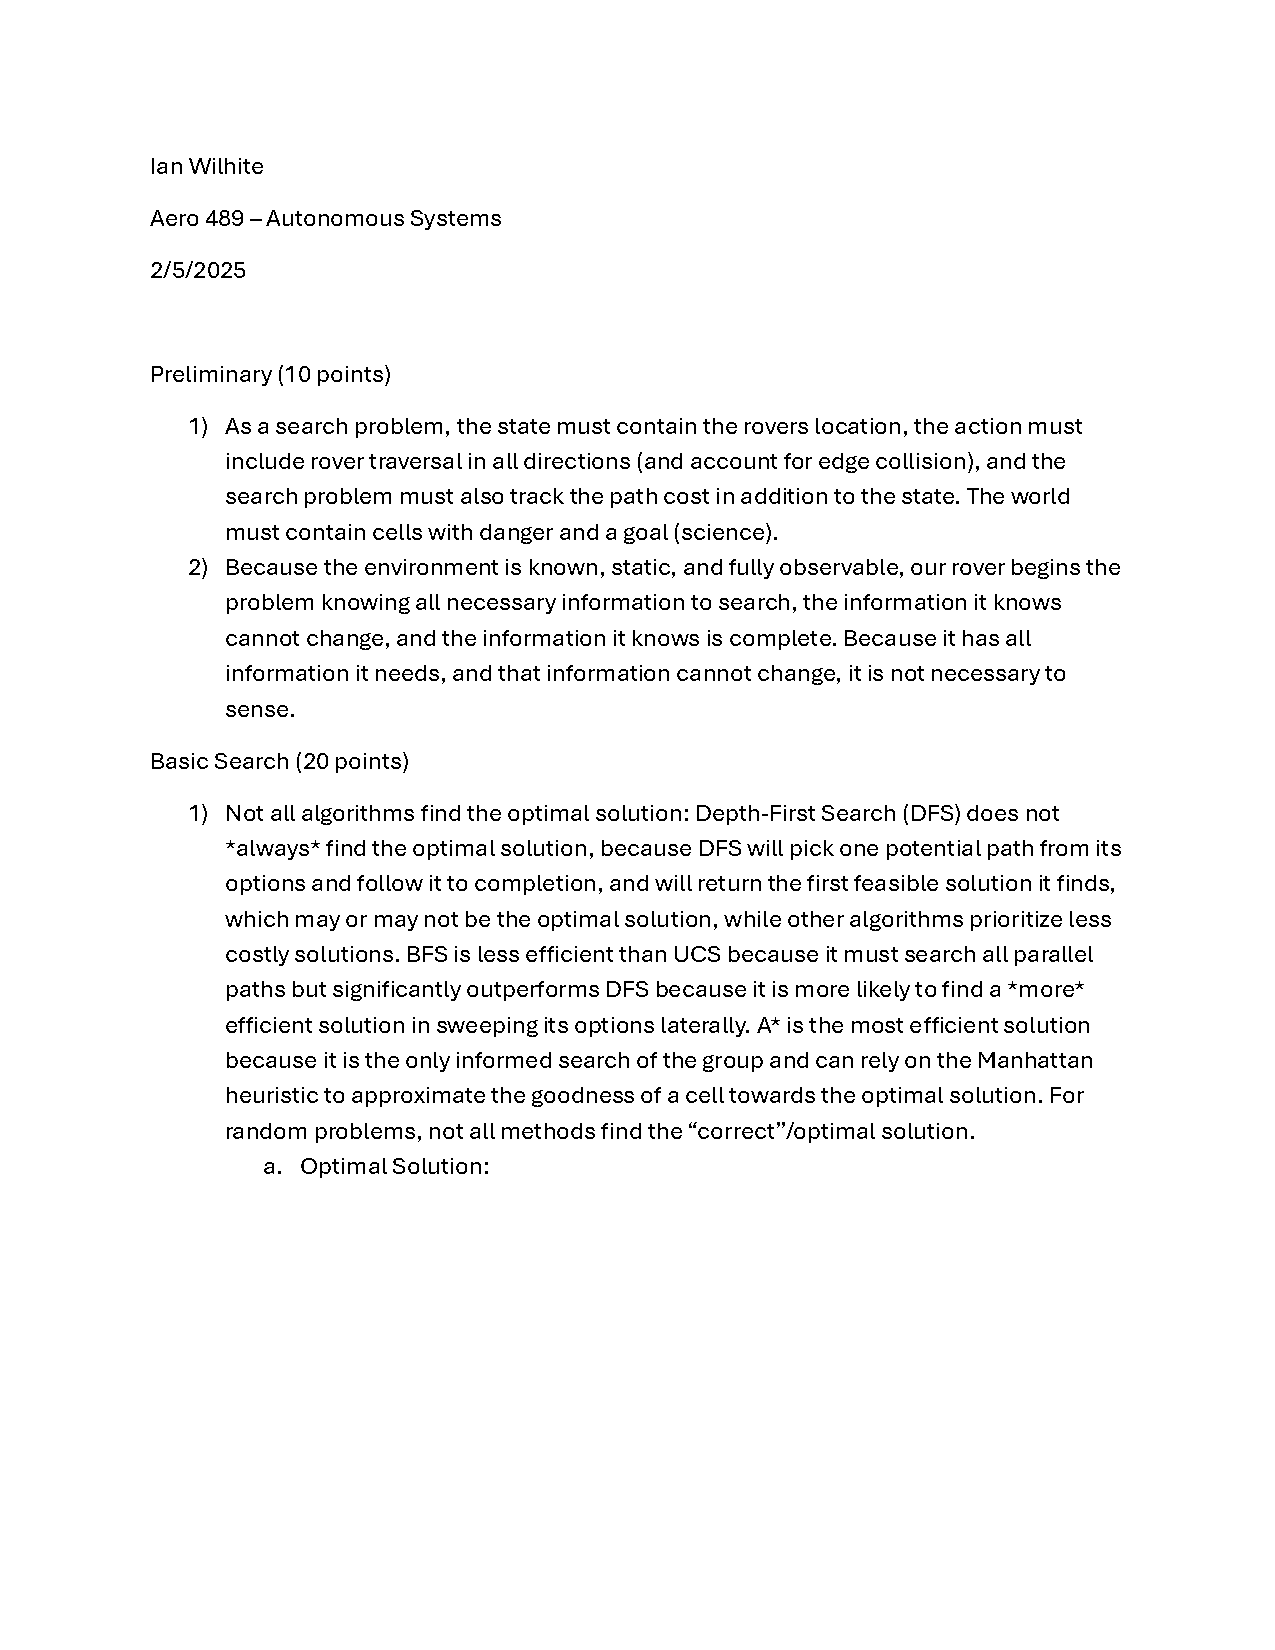
\includepdf[pages=-]{\detokenize{Resources/aero-489/aero-489-hw1.pdf}}
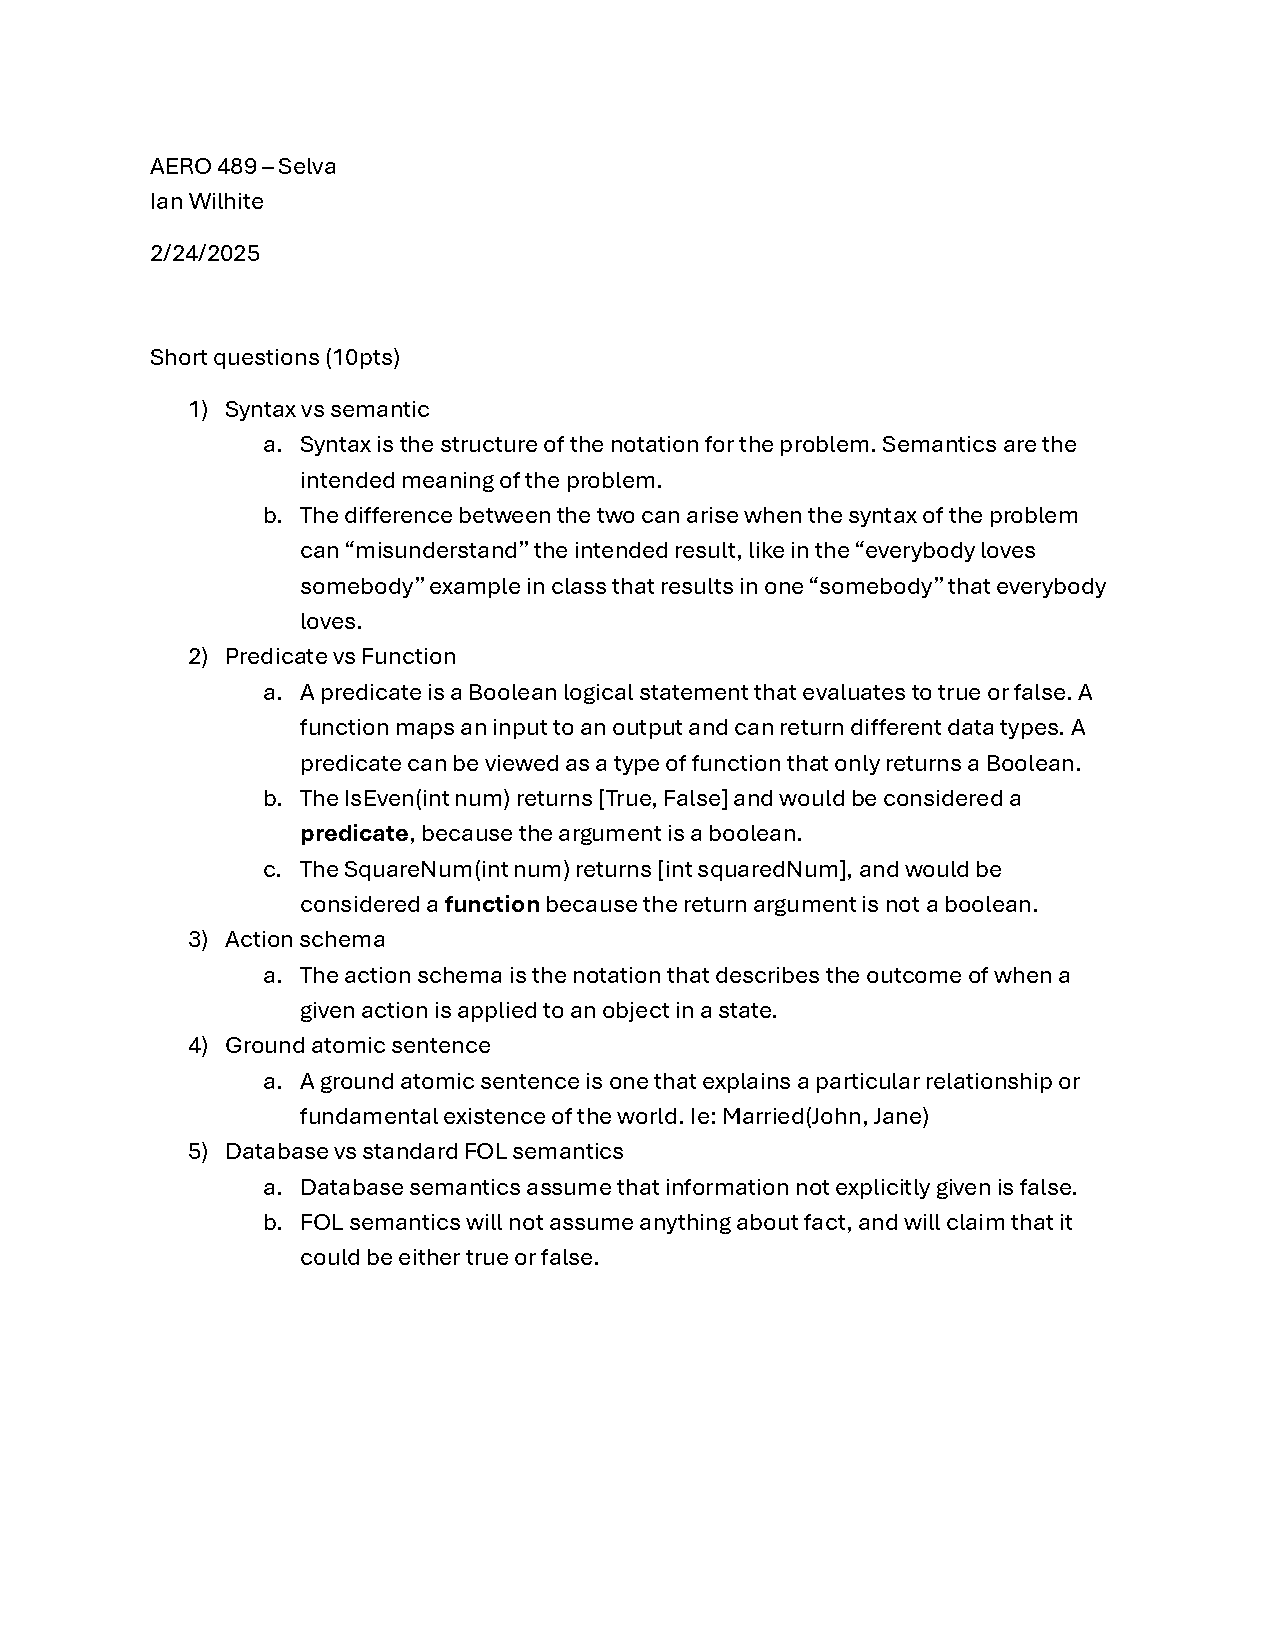
\includepdf[pages=-]{\detokenize{Resources/aero-489/aero-489-hw2.pdf}}
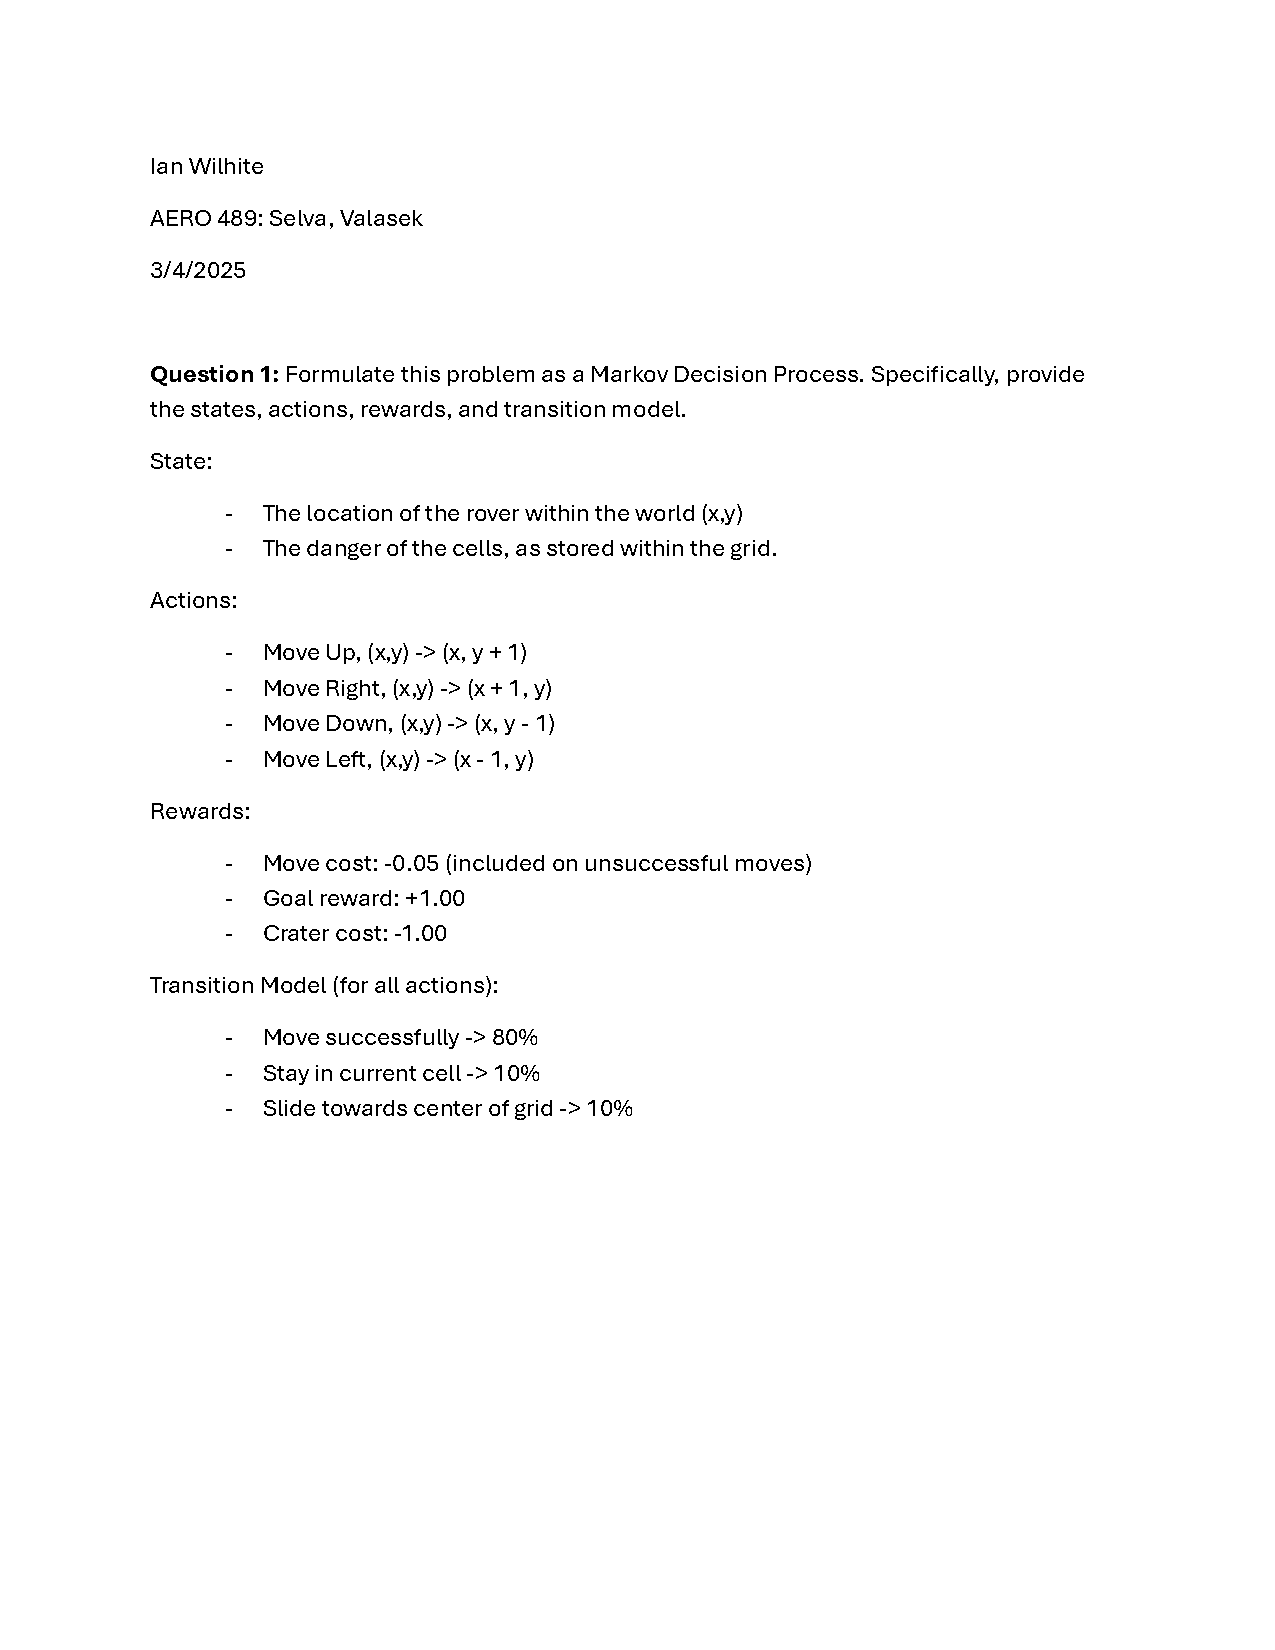
\includepdf[pages=-]{\detokenize{Resources/aero-489/aero-489-hw3.pdf}}
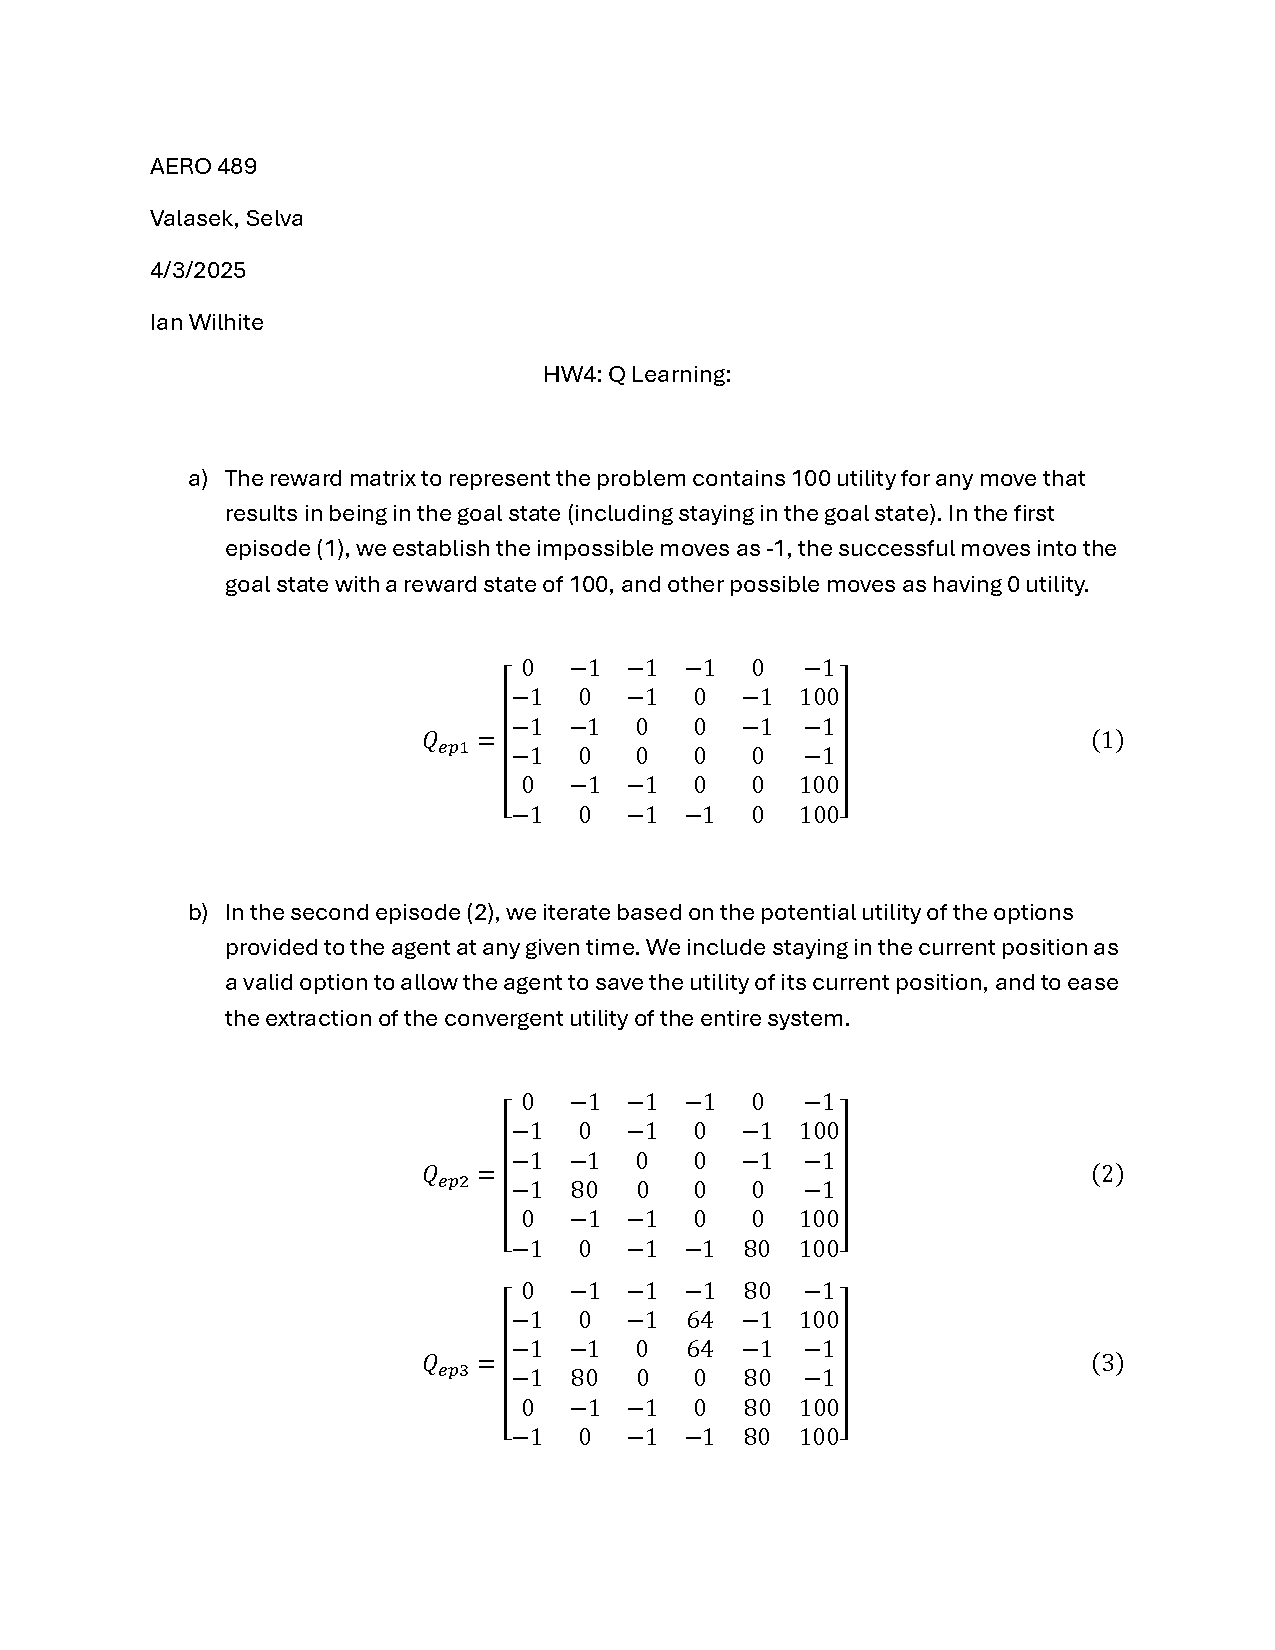
\includepdf[pages=-]{\detokenize{Resources/aero-489/aero-489-hw4.pdf}}
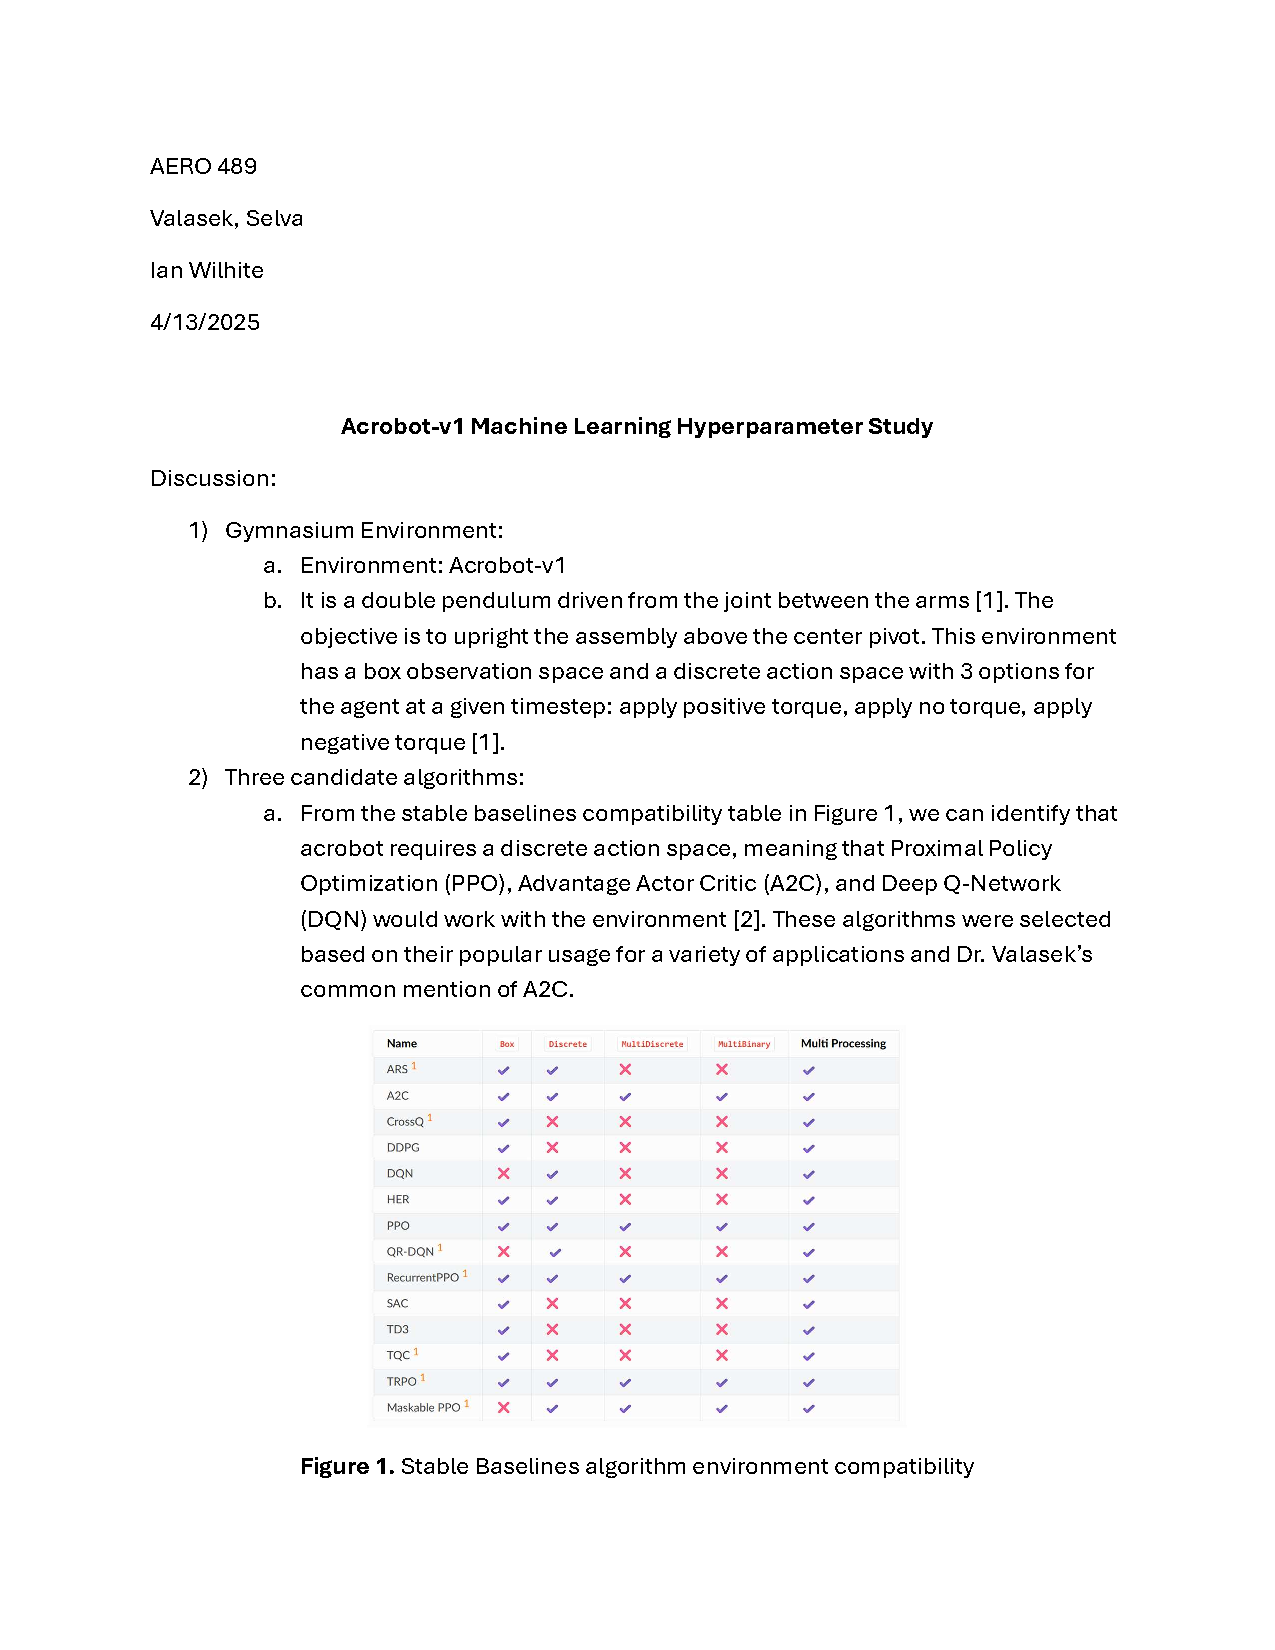
\includepdf[pages=-]{\detokenize{Resources/aero-489/aero-489-hw5.pdf}}
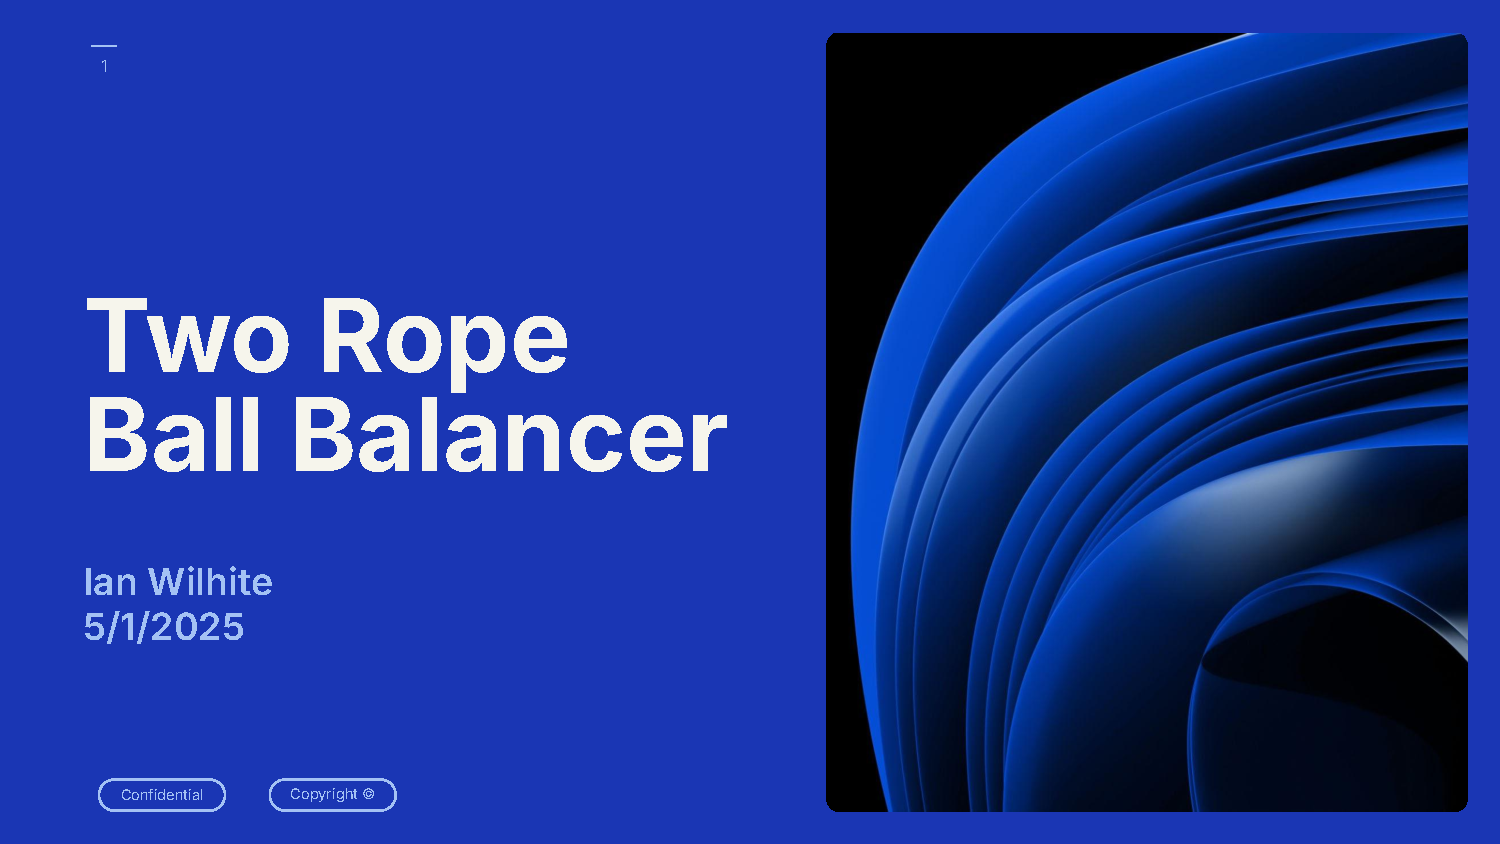
\includepdf[pages=-, landscape]{\detokenize{Resources/aero-489/AERO_489_final_presentation.pdf}}
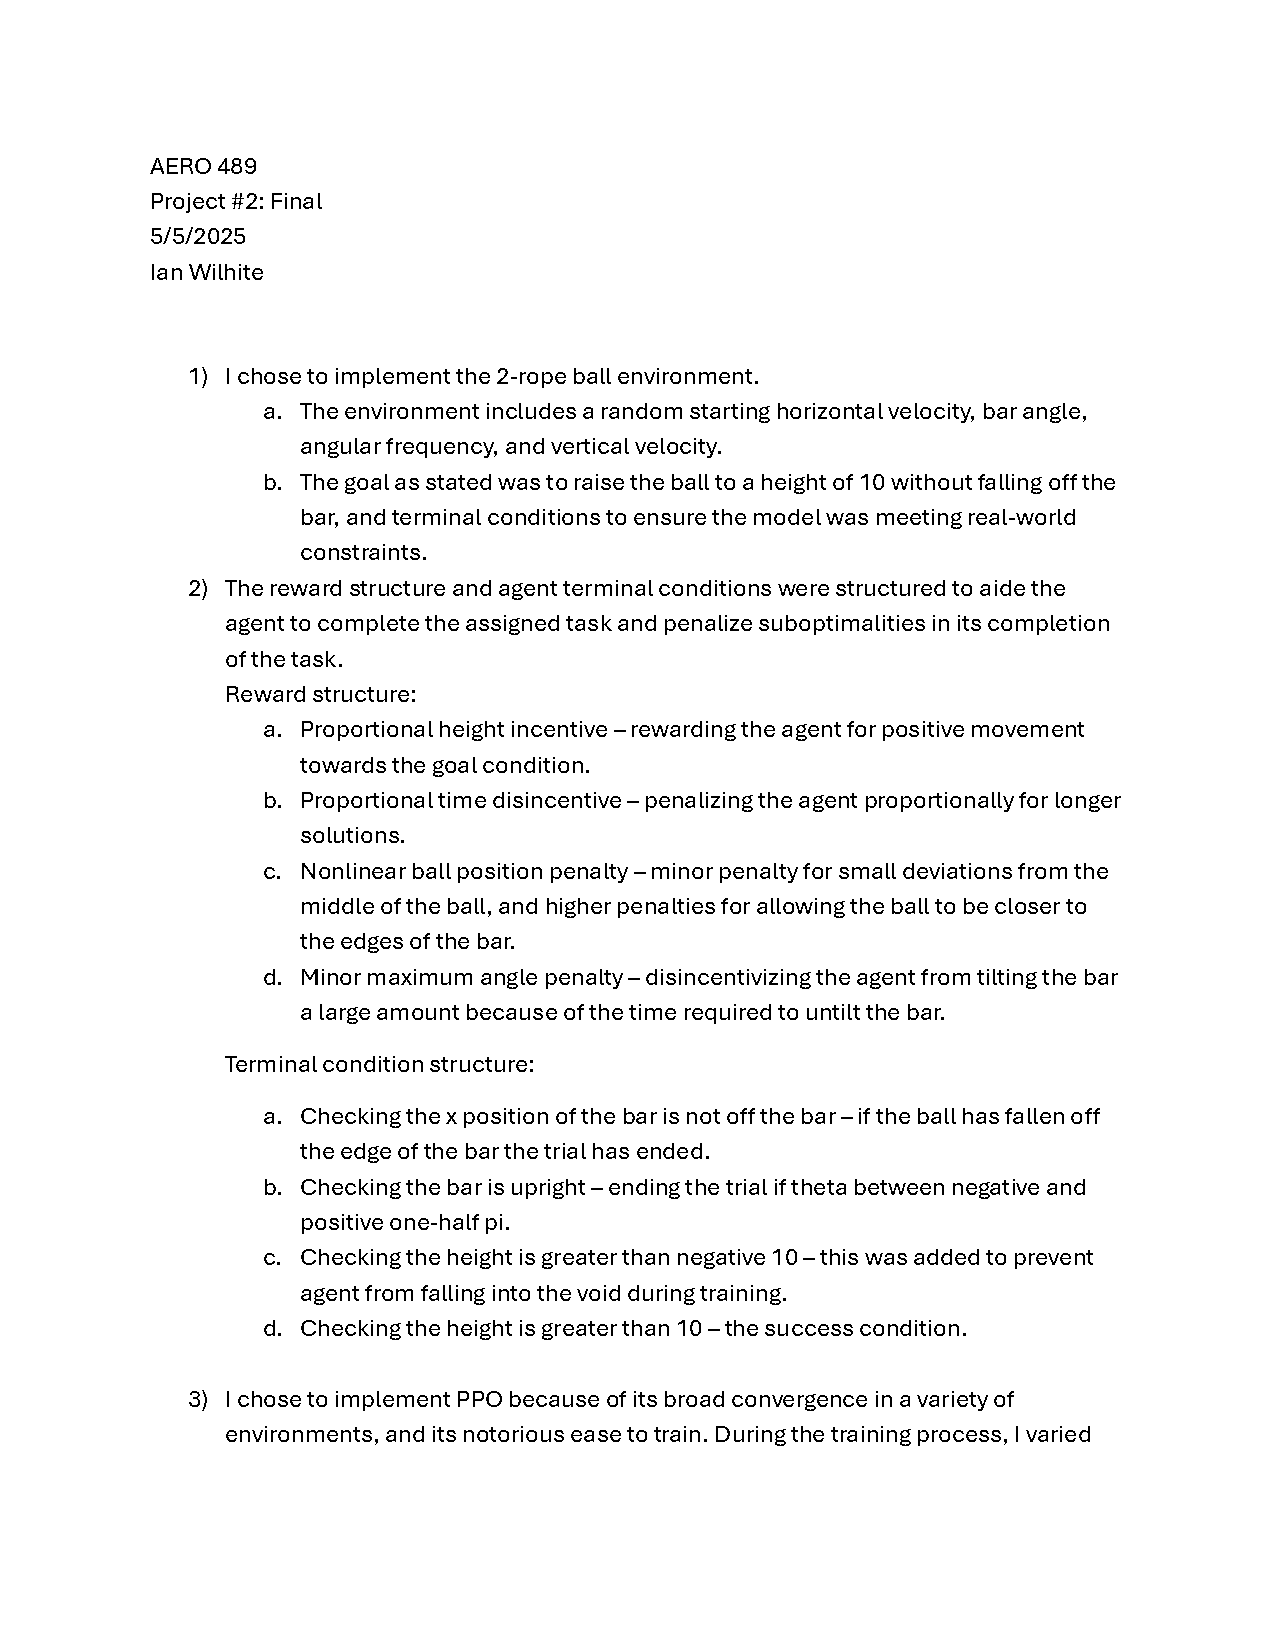
\includepdf[pages=-]{\detokenize{Resources/aero-489/aero-489-Final.pdf}}

\hyperlink{toc}{Back to Contents}
\section{Dynamics and Vibrations}
\subsection*{Summary}
\textbf{Content:} This section contains projects from an undergraduate dynamics course evaluating dynamic problems, modeling approaches, and foundational physical simulation.  
\begin{itemize}
    \item P1: Bungee Jumping
    \item P2: Piston Kinematics
    \item P3: Mixer Torques \& Kinematics
\end{itemize}
\textbf{Contributors:} Tori Abell, Alois Campbell, Jake Smith, Eddy Silva, Ian Wilhite

\textbf{Key Skills:} Dynamics, Vibrations, System Modeling, Validation, and Technical Writing.

\textbf{Relevance:} The projects emphasize direct conclusions based on experimental results. In these works, I often worked to write the code for the simulations and generate the charts to represent the teams findings. 

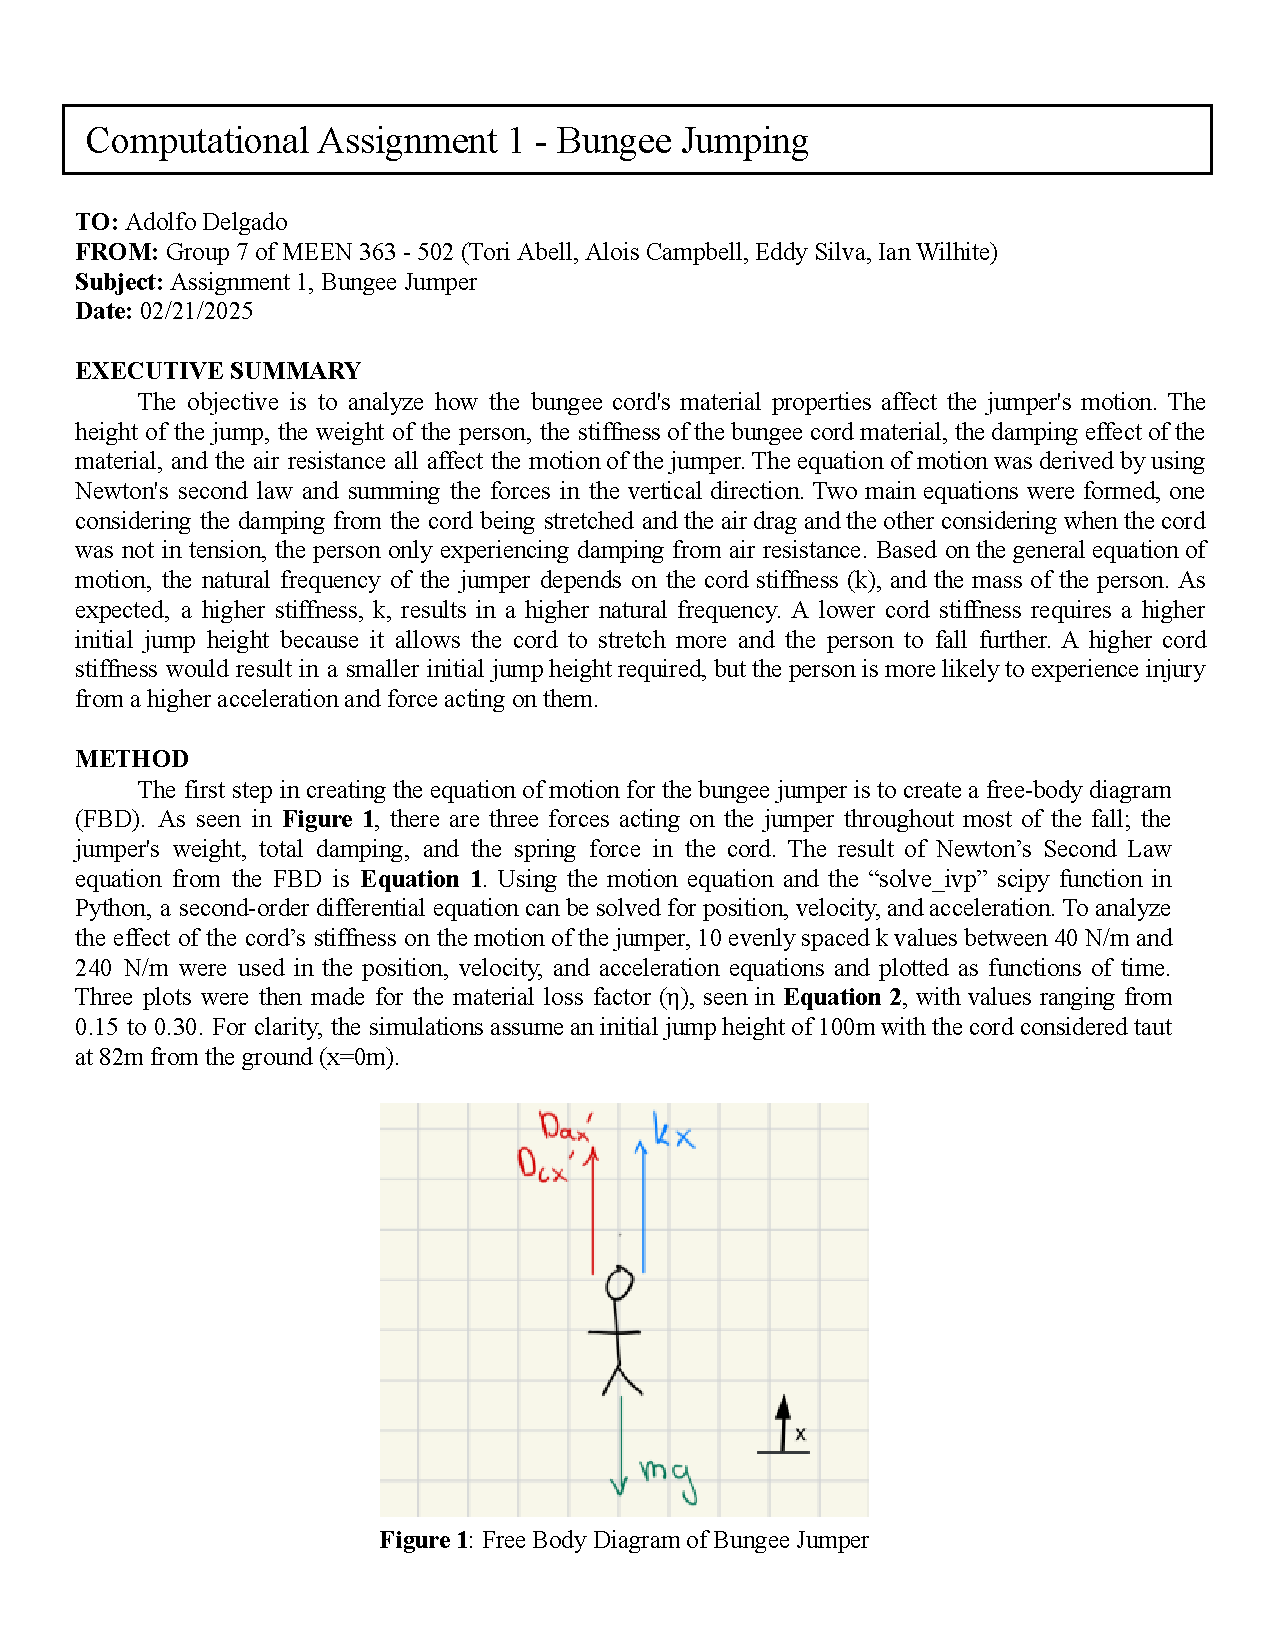
\includepdf[pages=-]{\detokenize{Resources/meen-363/meen-363-1_Group7.pdf}}
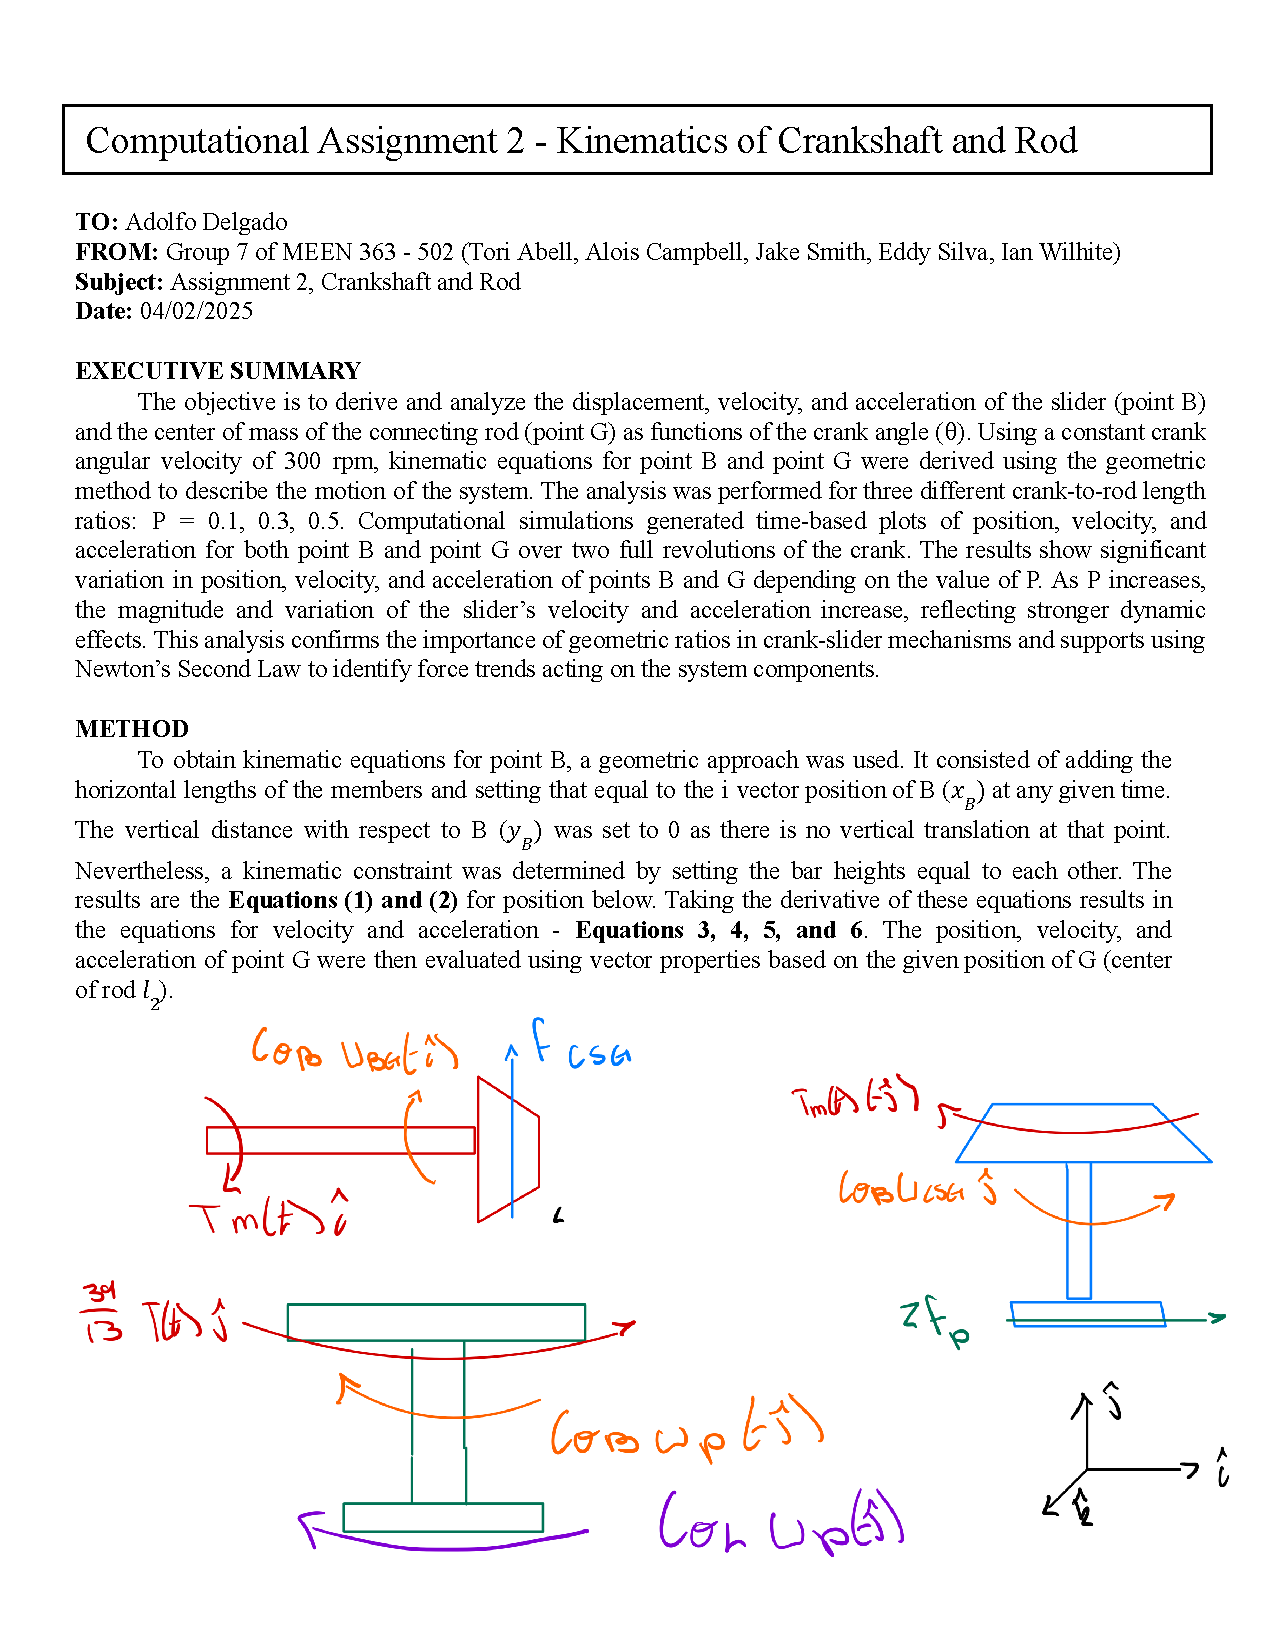
\includepdf[pages=-]{\detokenize{Resources/meen-363/meen-363-2_Group7.pdf}}
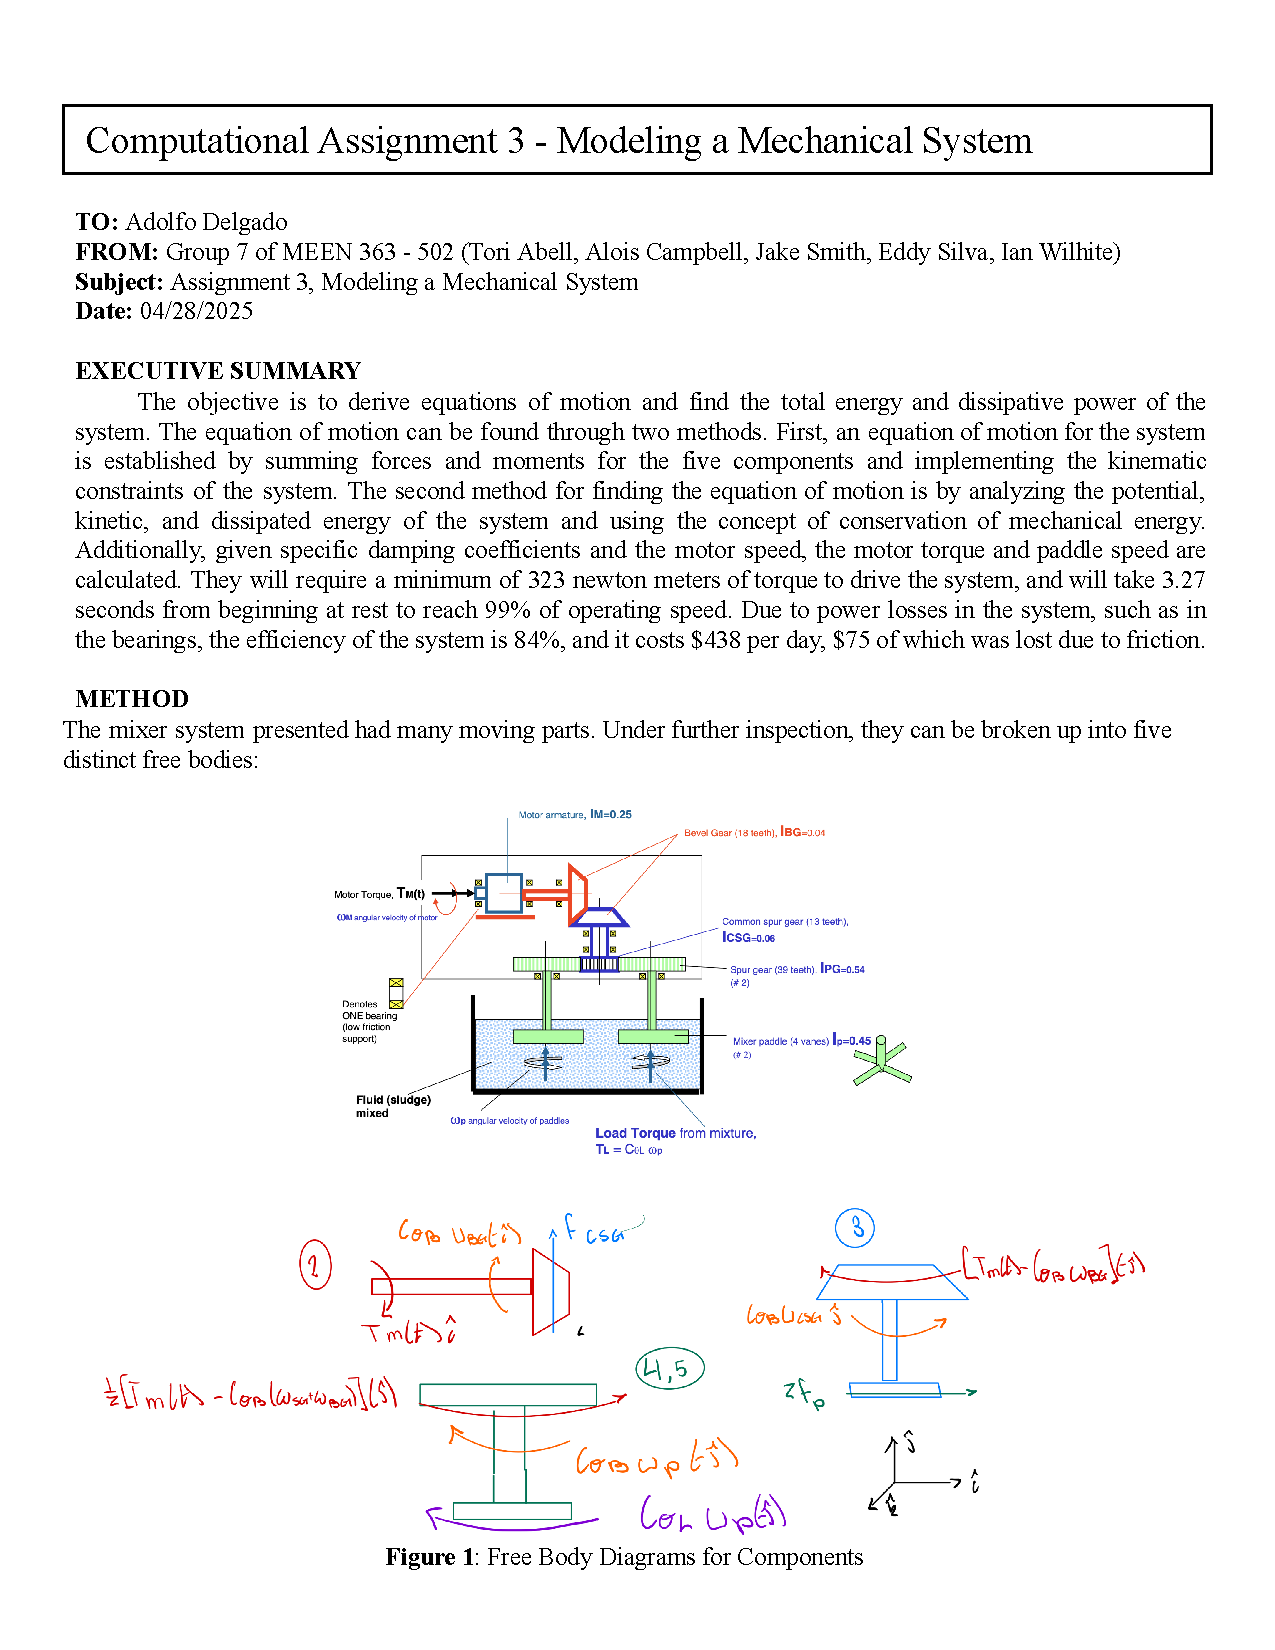
\includepdf[pages=-]{\detokenize{Resources/meen-363/meen-363-3_Group7.pdf}}

\hyperlink{toc}{Back to Contents}
\section{Numerical Methods (4th Place in Final Competition)}
\subsection*{Summary}
\textbf{Content:} This section includes four project phases from the Numerical Methods course (MEEN 357), in which we placed 4th of ~20 teams.
\begin{itemize}
    \item Phase 1: Foundations \& Subfunctions
    \item Phase 2: System Verification \& Analysis
    \item Phase 3: Parameter Validation \& Strategic Approach
    \item Phase 4: Final Competition Submission (Document)
\end{itemize}
\textbf{Contributors:} Jacob Hargreaves, Ian Wilhite, David Guess

\textbf{Key Skills:} Numerical Methods, Computational Analysis, Algorithm Development, Software Development, and Convex Optimization.

\textbf{Relevance:} This work demonstrates the development and management of large codebases, iterative verification and validation, and system design struture. 

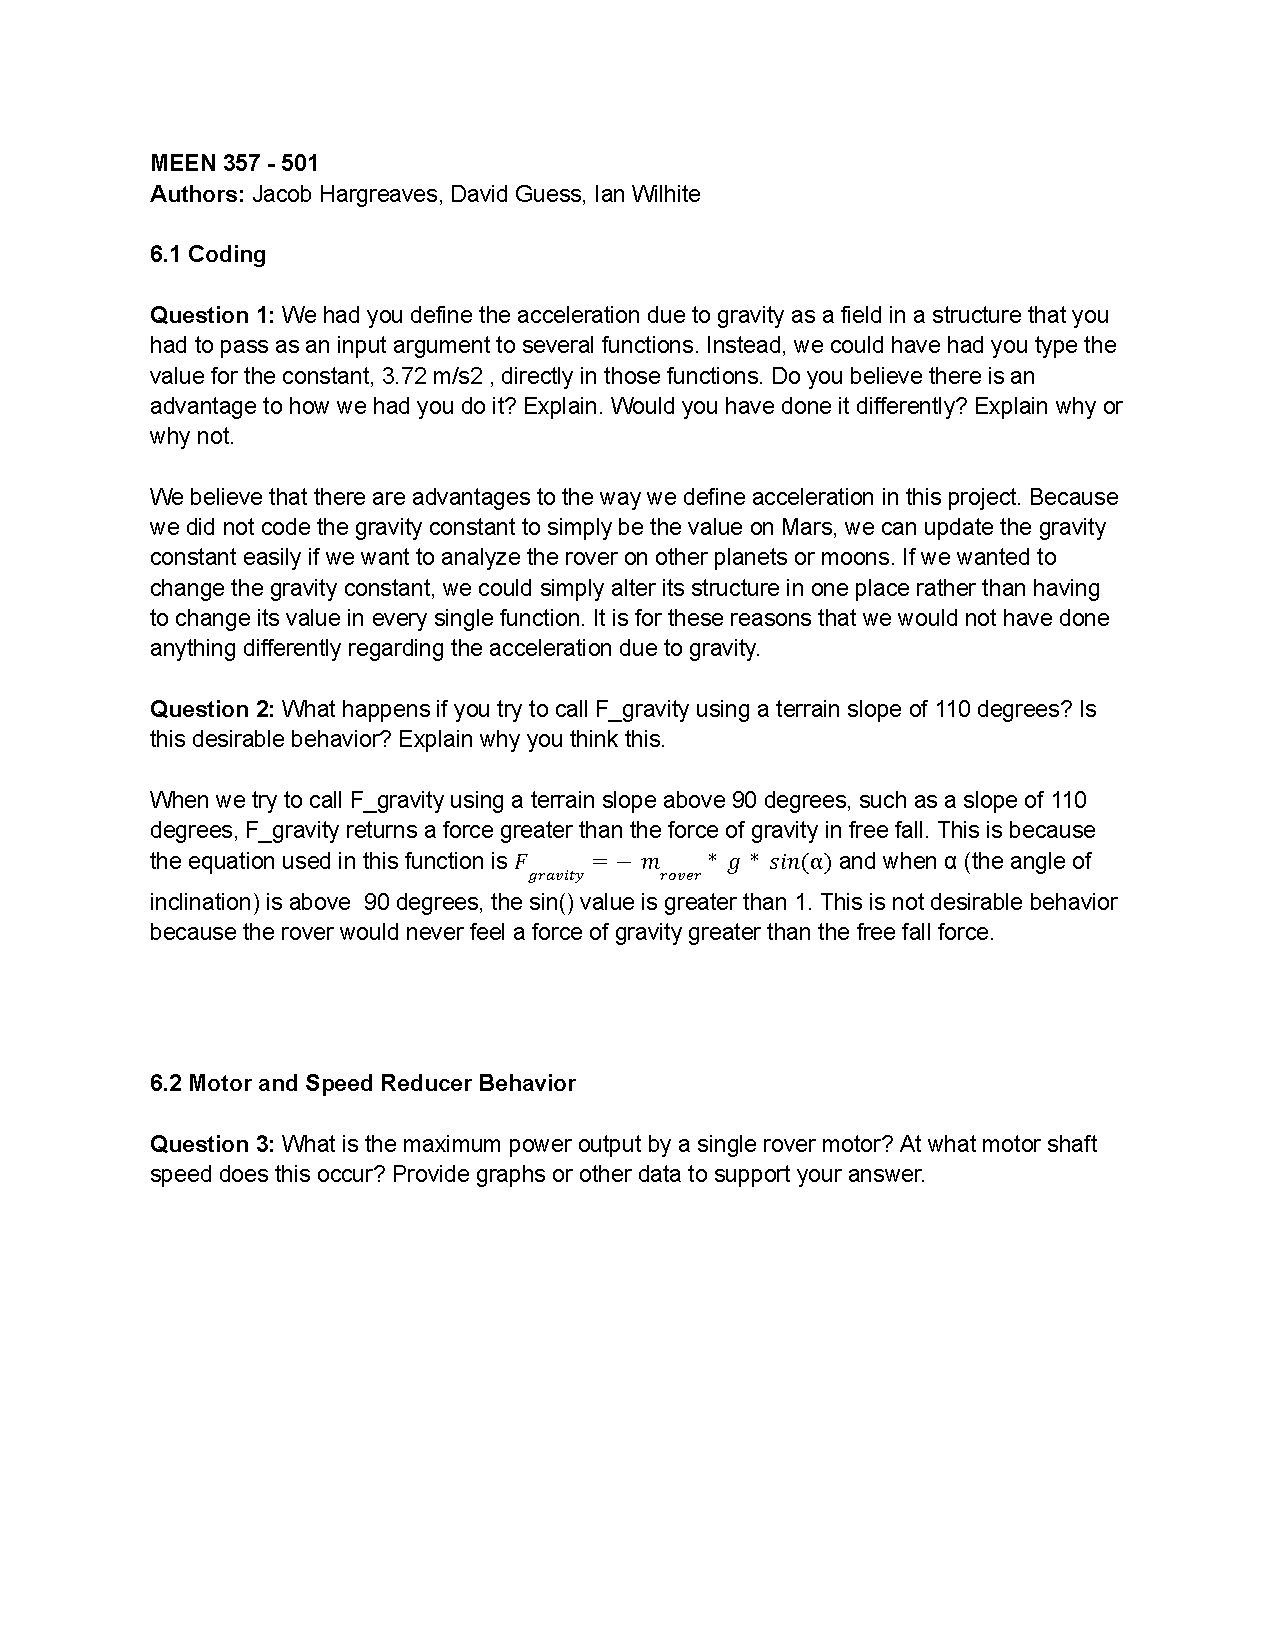
\includepdf[pages=-]{\detokenize{Resources/meen-357/meen-357-phase-1.pdf}}
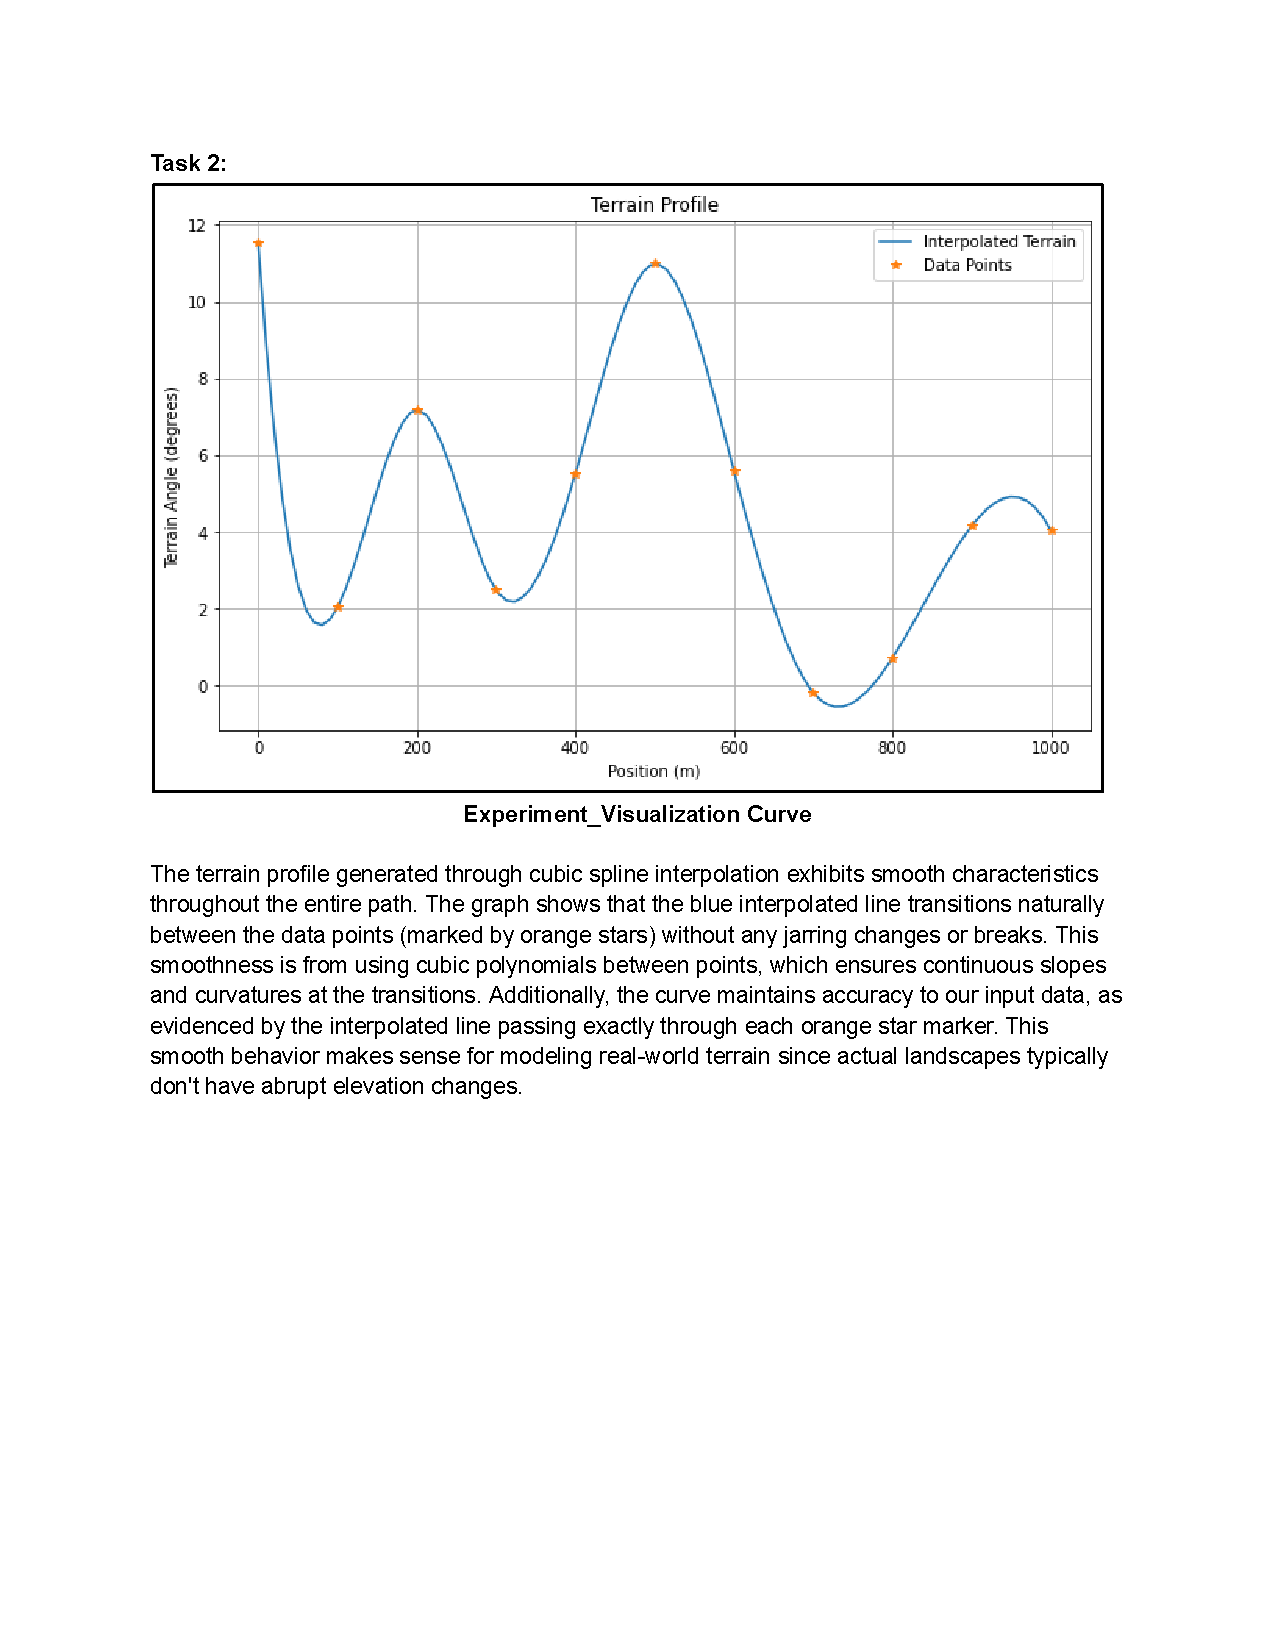
\includepdf[pages=-]{\detokenize{Resources/meen-357/meen-357-phase-2.pdf}}
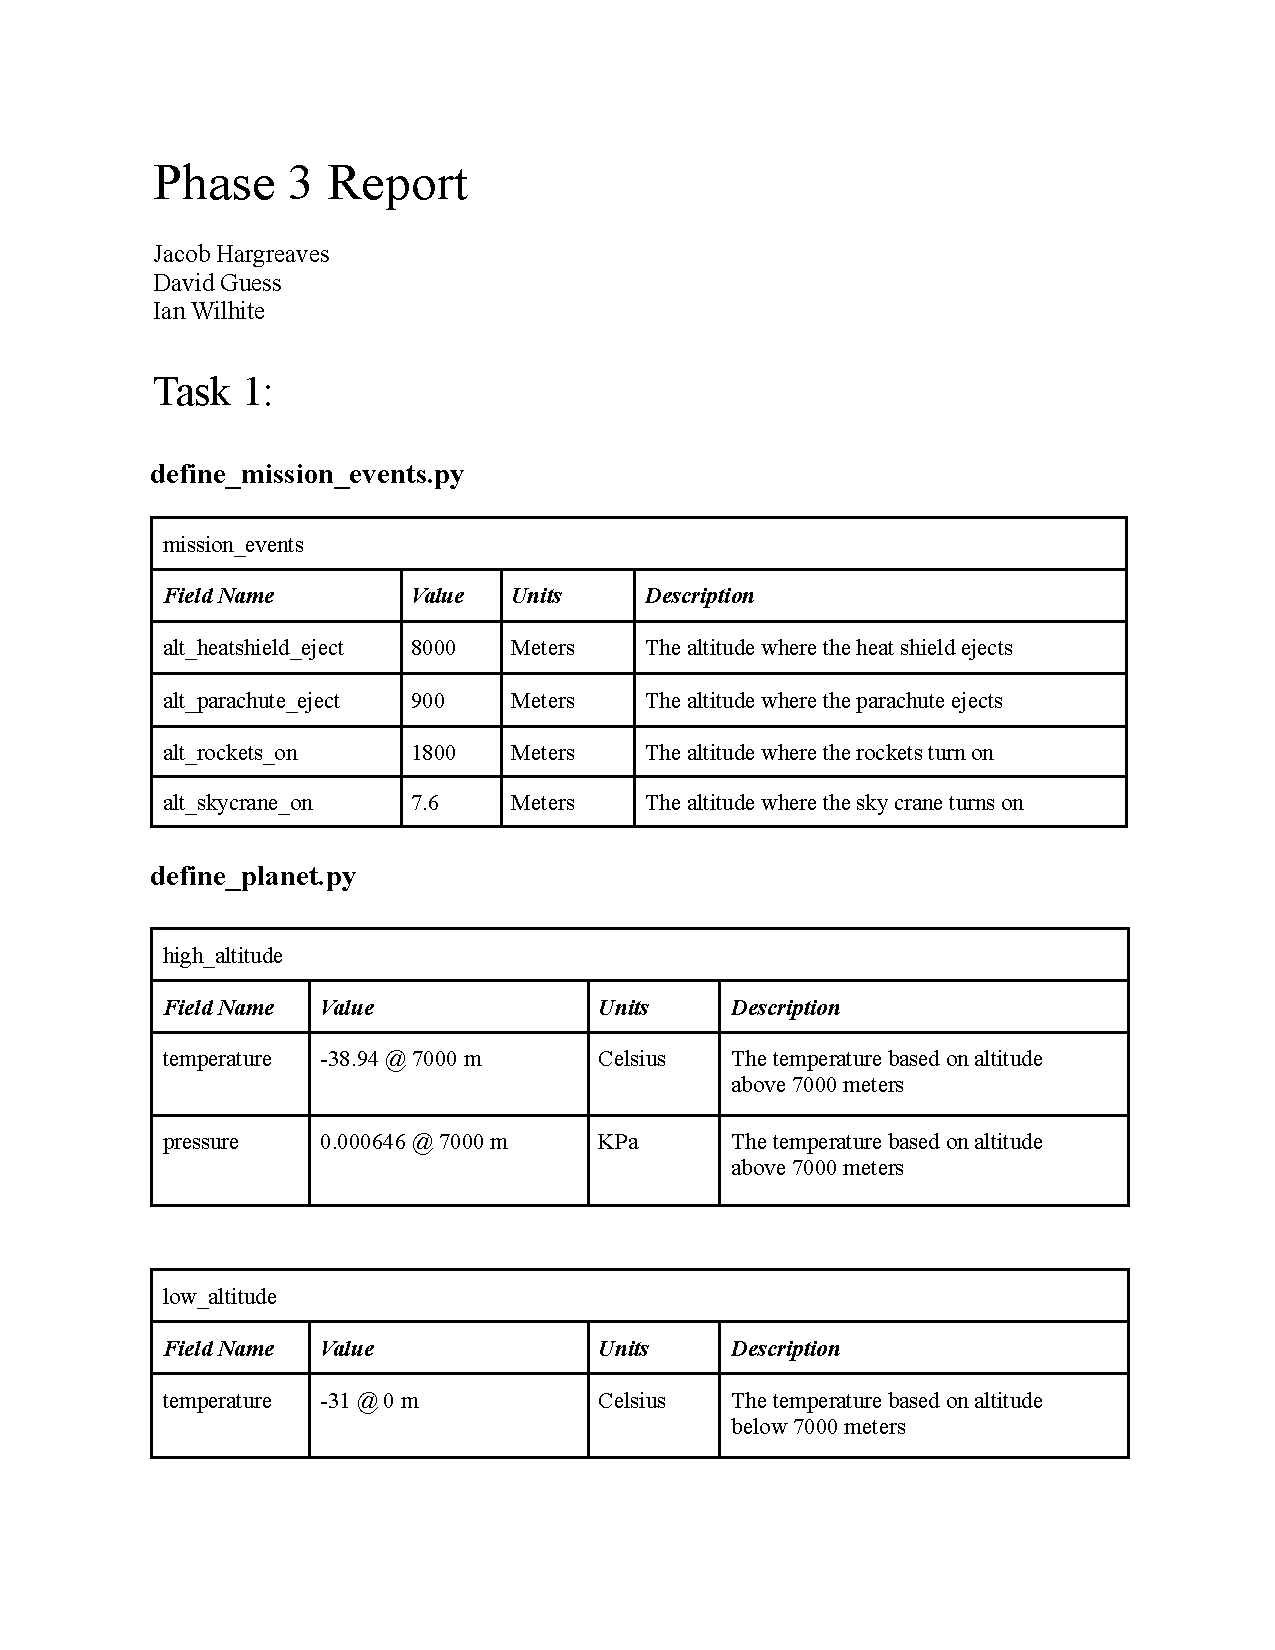
\includepdf[pages=-]{\detokenize{Resources/meen-357/meen-357-phase-3.pdf}}
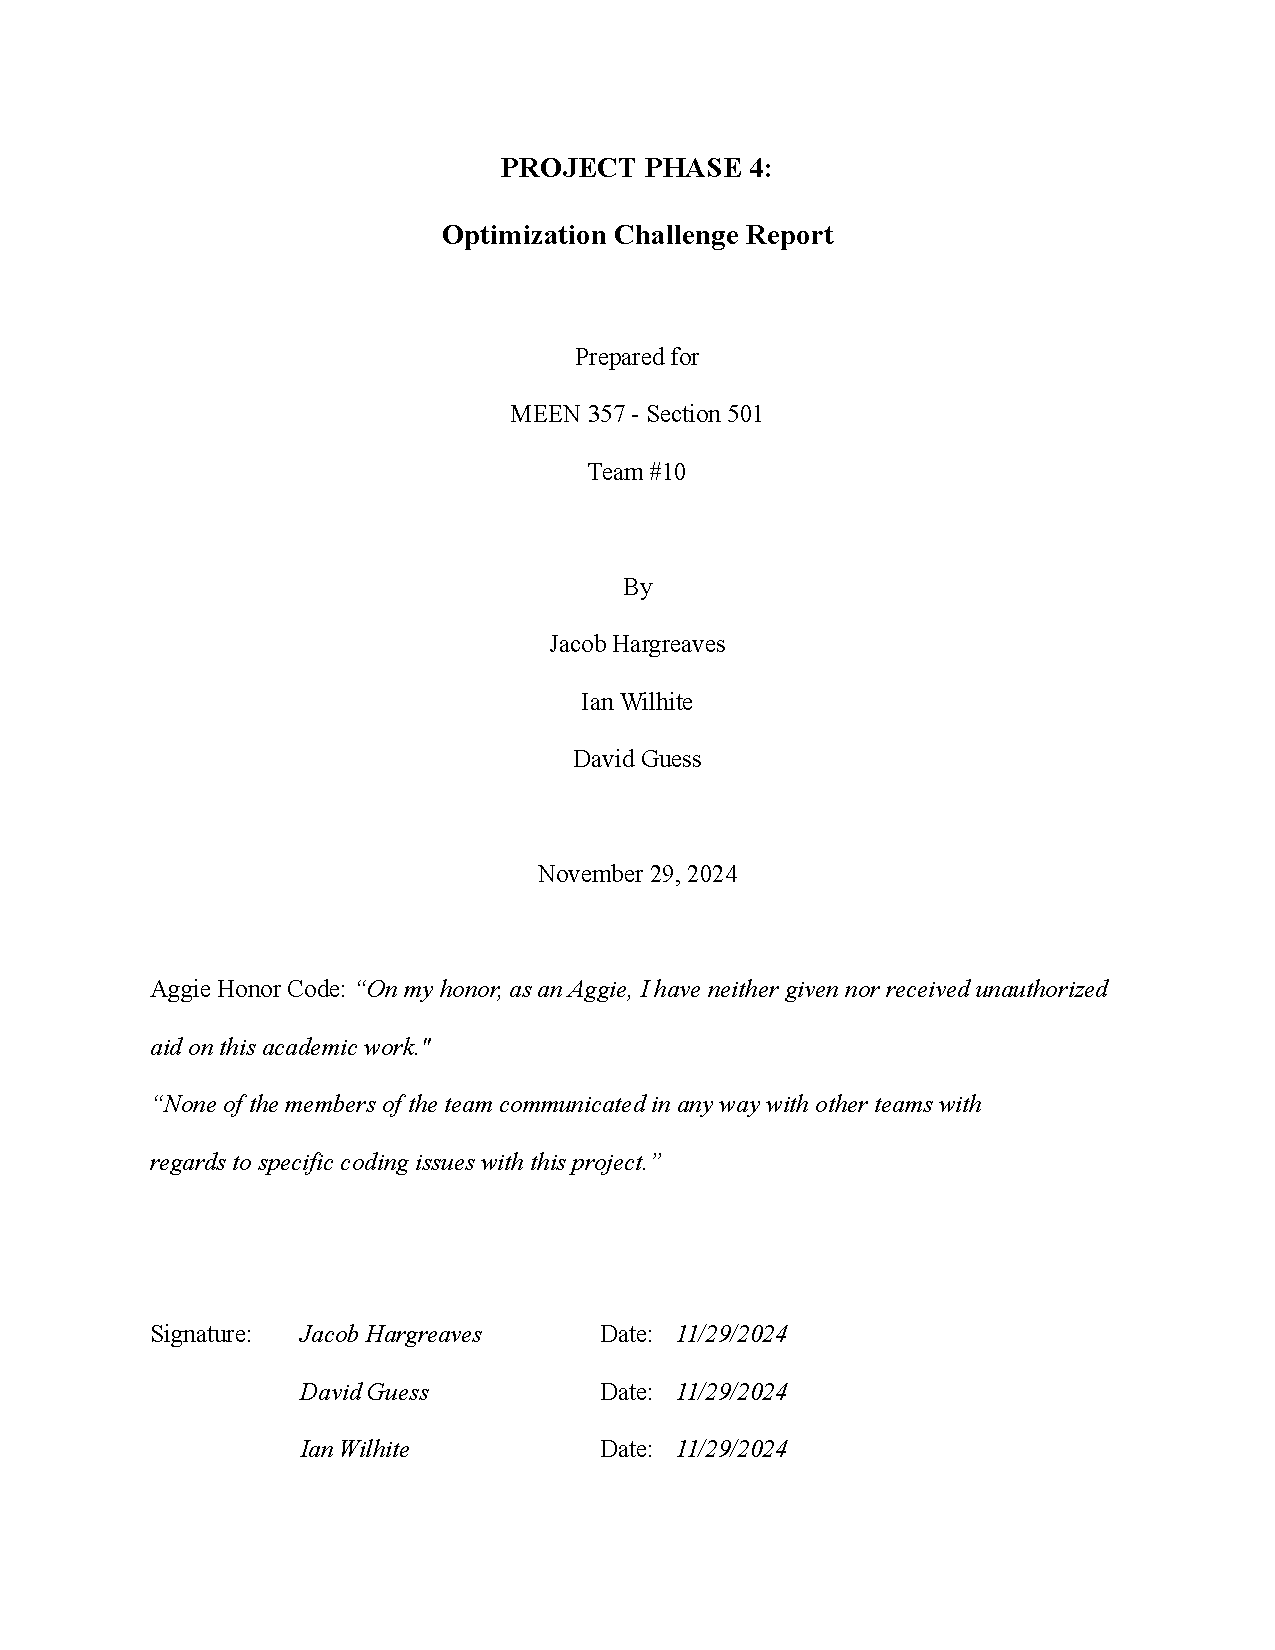
\includepdf[pages=-]{\detokenize{Resources/meen-357/meen-357-phase-4.pdf}}

\hyperlink{toc}{Back to Contents}
\section{SEC Ignite Competition (3rd Place)}
\subsection*{Summary}
\textbf{Content:} This section features the presentation from the SEC Ignite Competition, where my team achieved 3rd place.
\begin{itemize}
    \item AM5\_2024.pdf
\end{itemize}
\textbf{Contributors:} 

\textbf{Key Skills:} Innovation, Entrepreneurship, Public Speaking, Pitching, Business Model Development, Teamwork.

\textbf{Relevance:} This presentation demonstrates strong communication and entrepreneurial skills, and the ability to develop and articulate a compelling business case for a technical innovation in a competitive setting.

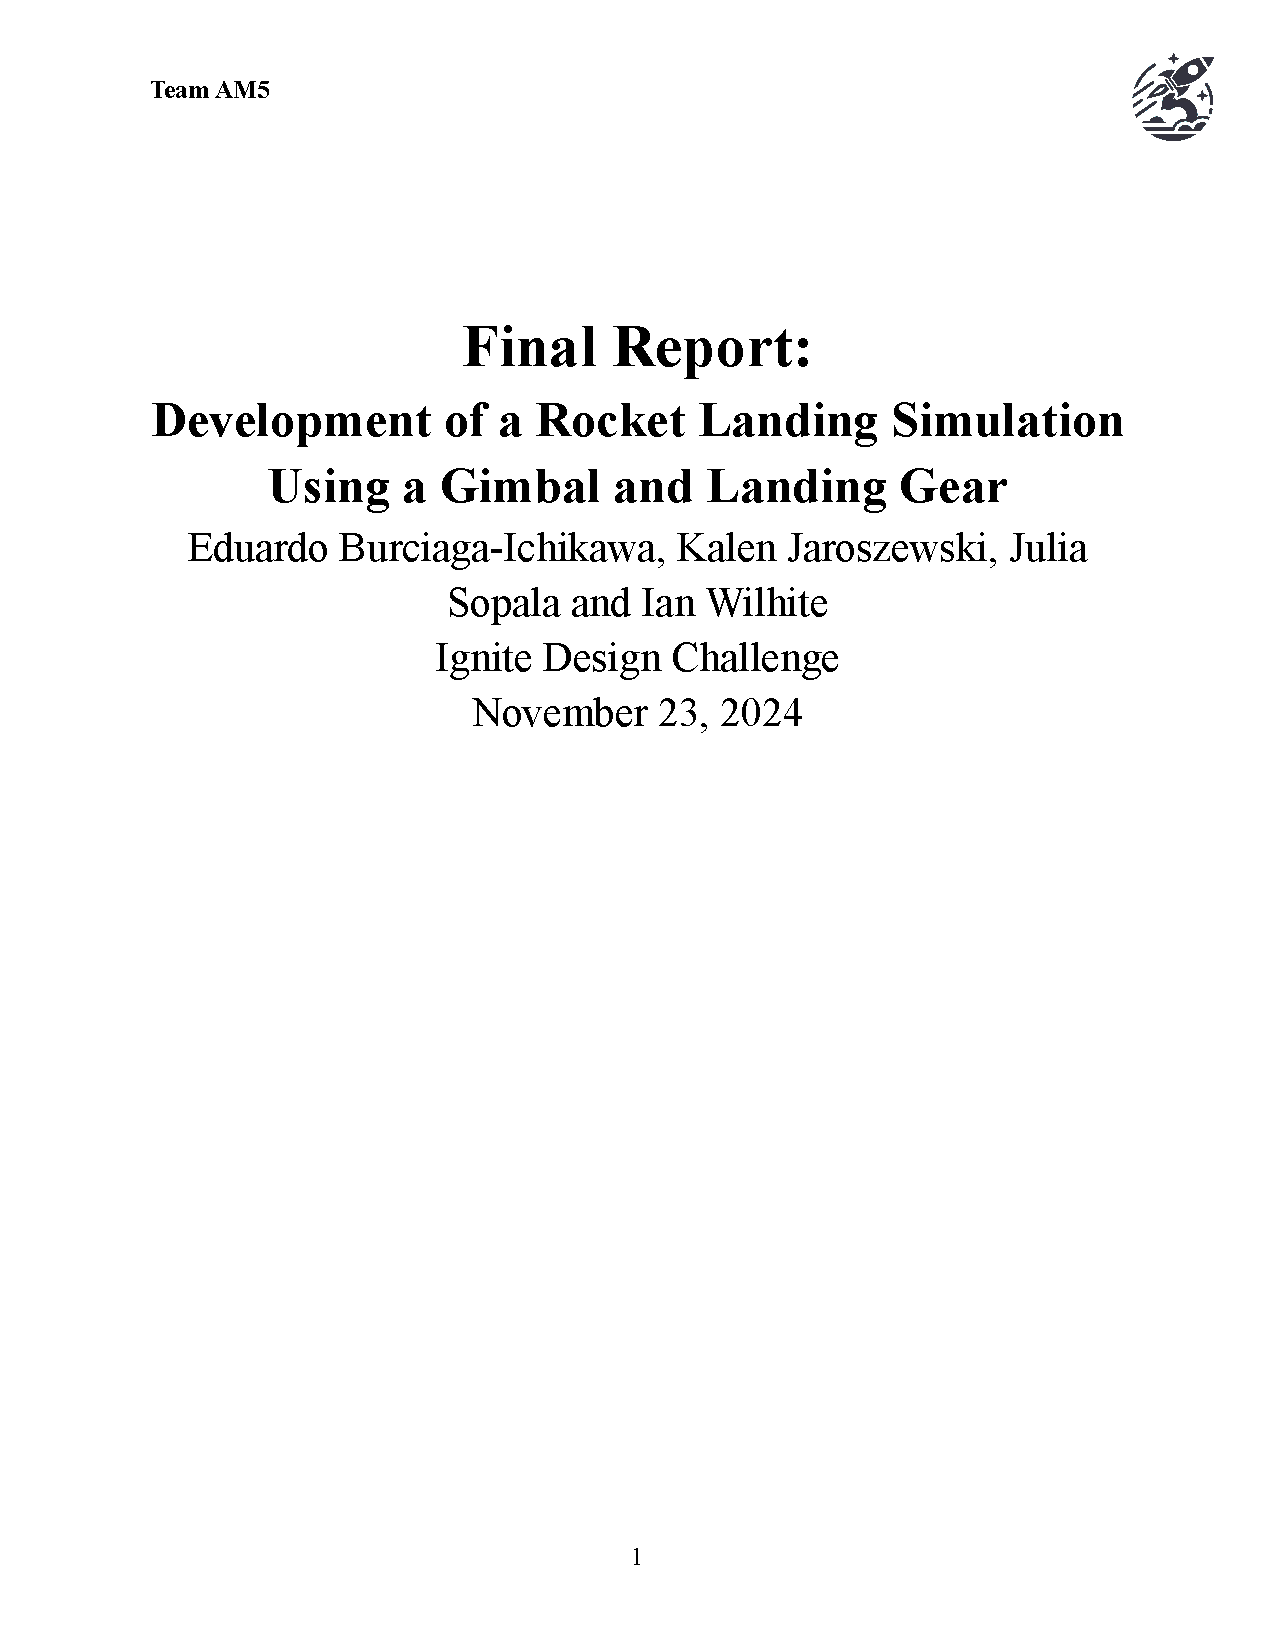
\includepdf[pages=-]{\detokenize{Resources/sec-ignite/AM5_2024.pdf}}

\hyperlink{toc}{Back to Contents}
\section{Mechanical Modeling}
\subsection*{Summary}
\textbf{Content:} This section presents the final project from the Mechanical Modeling course (MEEN 210).
\begin{itemize}
    \item meen-210-Final\_Project.pdf
\end{itemize}
\textbf{Contributors:} Ian Wilhite (Solo Project)

\textbf{Key Skills:} Mechanical Design, CAD, SolidWorks, Finite Element Analysis (FEA), 3D Modeling, Technical Drawing.

\textbf{Relevance:} This project showcases the ability to design, model, and analyze mechanical components and assemblies using industry-standard software. It reflects a strong understanding of mechanical design principles.

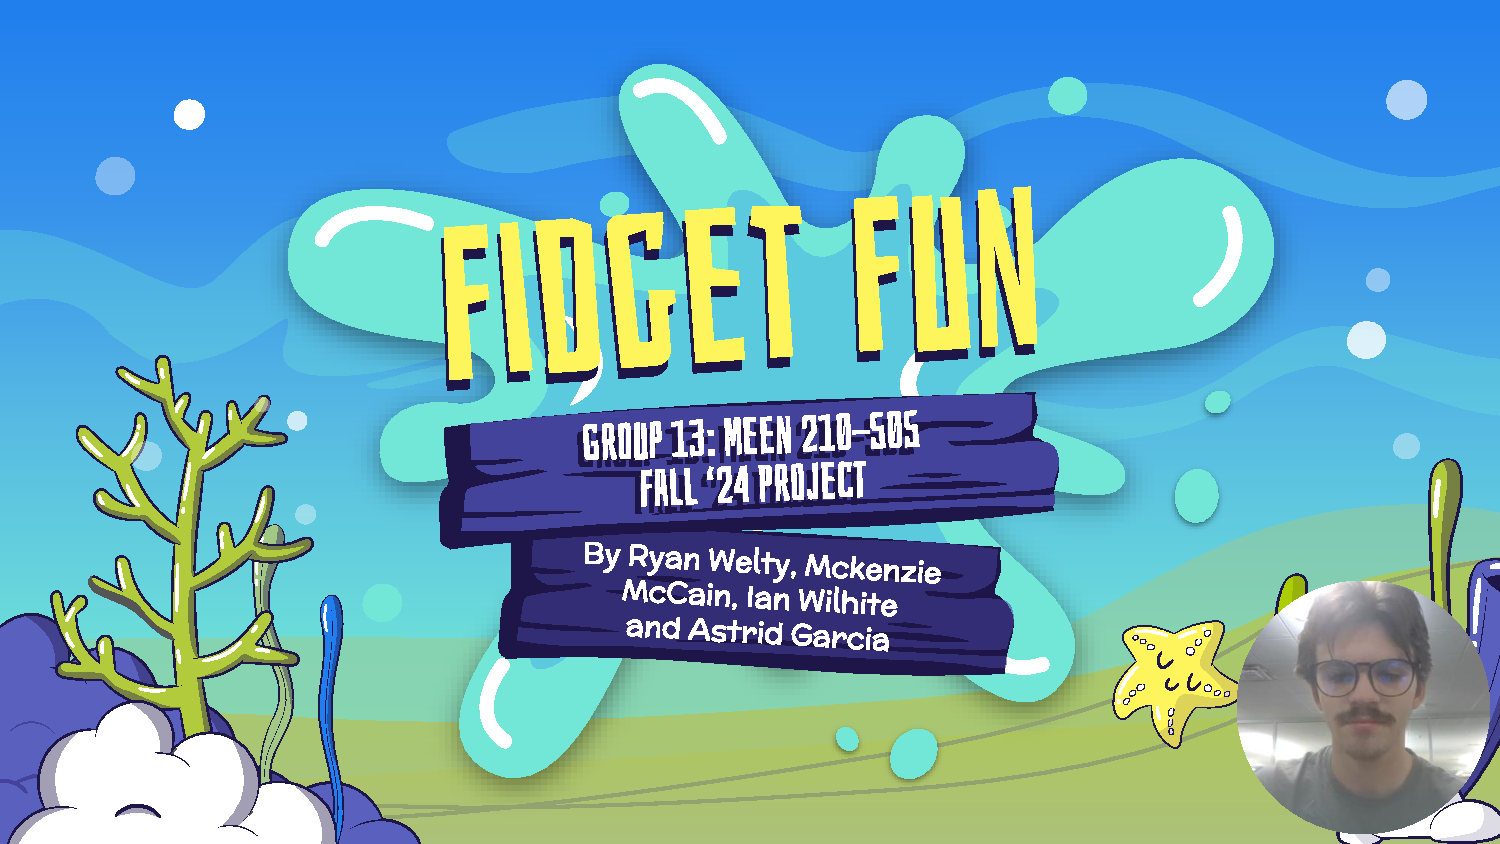
\includepdf[pages=-, landscape]{\detokenize{Resources/meen-210/meen-210-Final_Project.pdf}}

\hyperlink{toc}{Back to Contents}
\section{Mechanical Measurements}
\subsection*{Summary}
\textbf{Content:} This section includes a technical memorandum from the Mechanical Measurements course (MEEN 260).
\begin{itemize}
    \item meen-260-memo.pdf
\end{itemize}
\textbf{Contributors:} Ian Wilhite (Solo Project)

\textbf{Key Skills:} Data Acquisition, Instrumentation, Sensors, LabVIEW, Signal Processing, Technical Writing, Experimental Analysis.

\textbf{Relevance:} This document demonstrates hands-on experience with experimental setups, data acquisition systems, and the analysis and presentation of experimental results in a professional format.

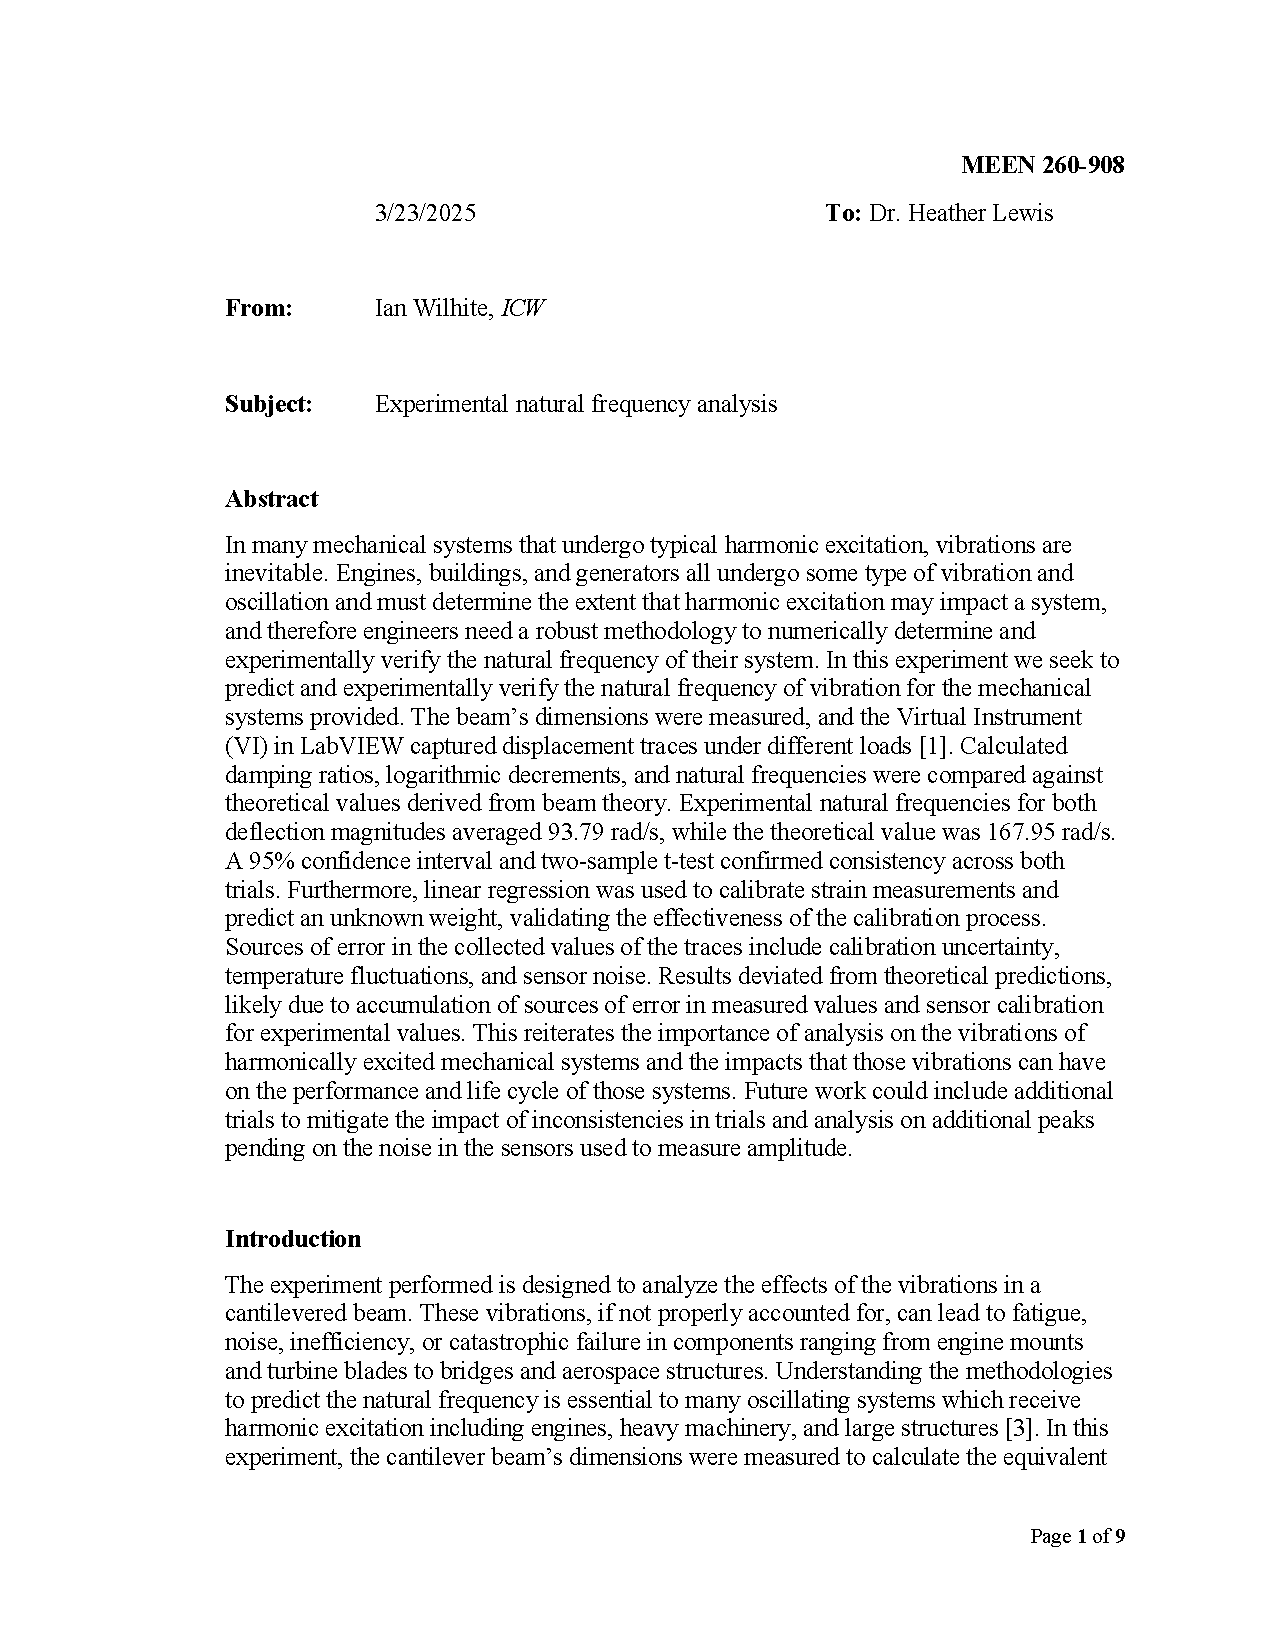
\includepdf[pages=-]{\detokenize{Resources/meen-260/meen-260-memo.pdf}}

\hyperlink{toc}{Back to Contents}
\section{Solid Mechanics}
\subsection*{Summary}
\textbf{Content:} This section contains two projects from the Solid Mechanics course (MEEN 305).
\begin{itemize}
    \item meen-305-Project\_1.pdf
    \item meen-305-Project\_2.pdf
\end{itemize}
\textbf{Contributors:} Ian Wilhite (Solo Project)

\textbf{Key Skills:} Solid Mechanics, Stress Analysis, Strain Analysis, Material Behavior, Finite Element Analysis (FEA), Structural Analysis.

\textbf{Relevance:} These projects demonstrate a solid understanding of the principles of solid mechanics and their application to the analysis of structural components under various loading conditions.

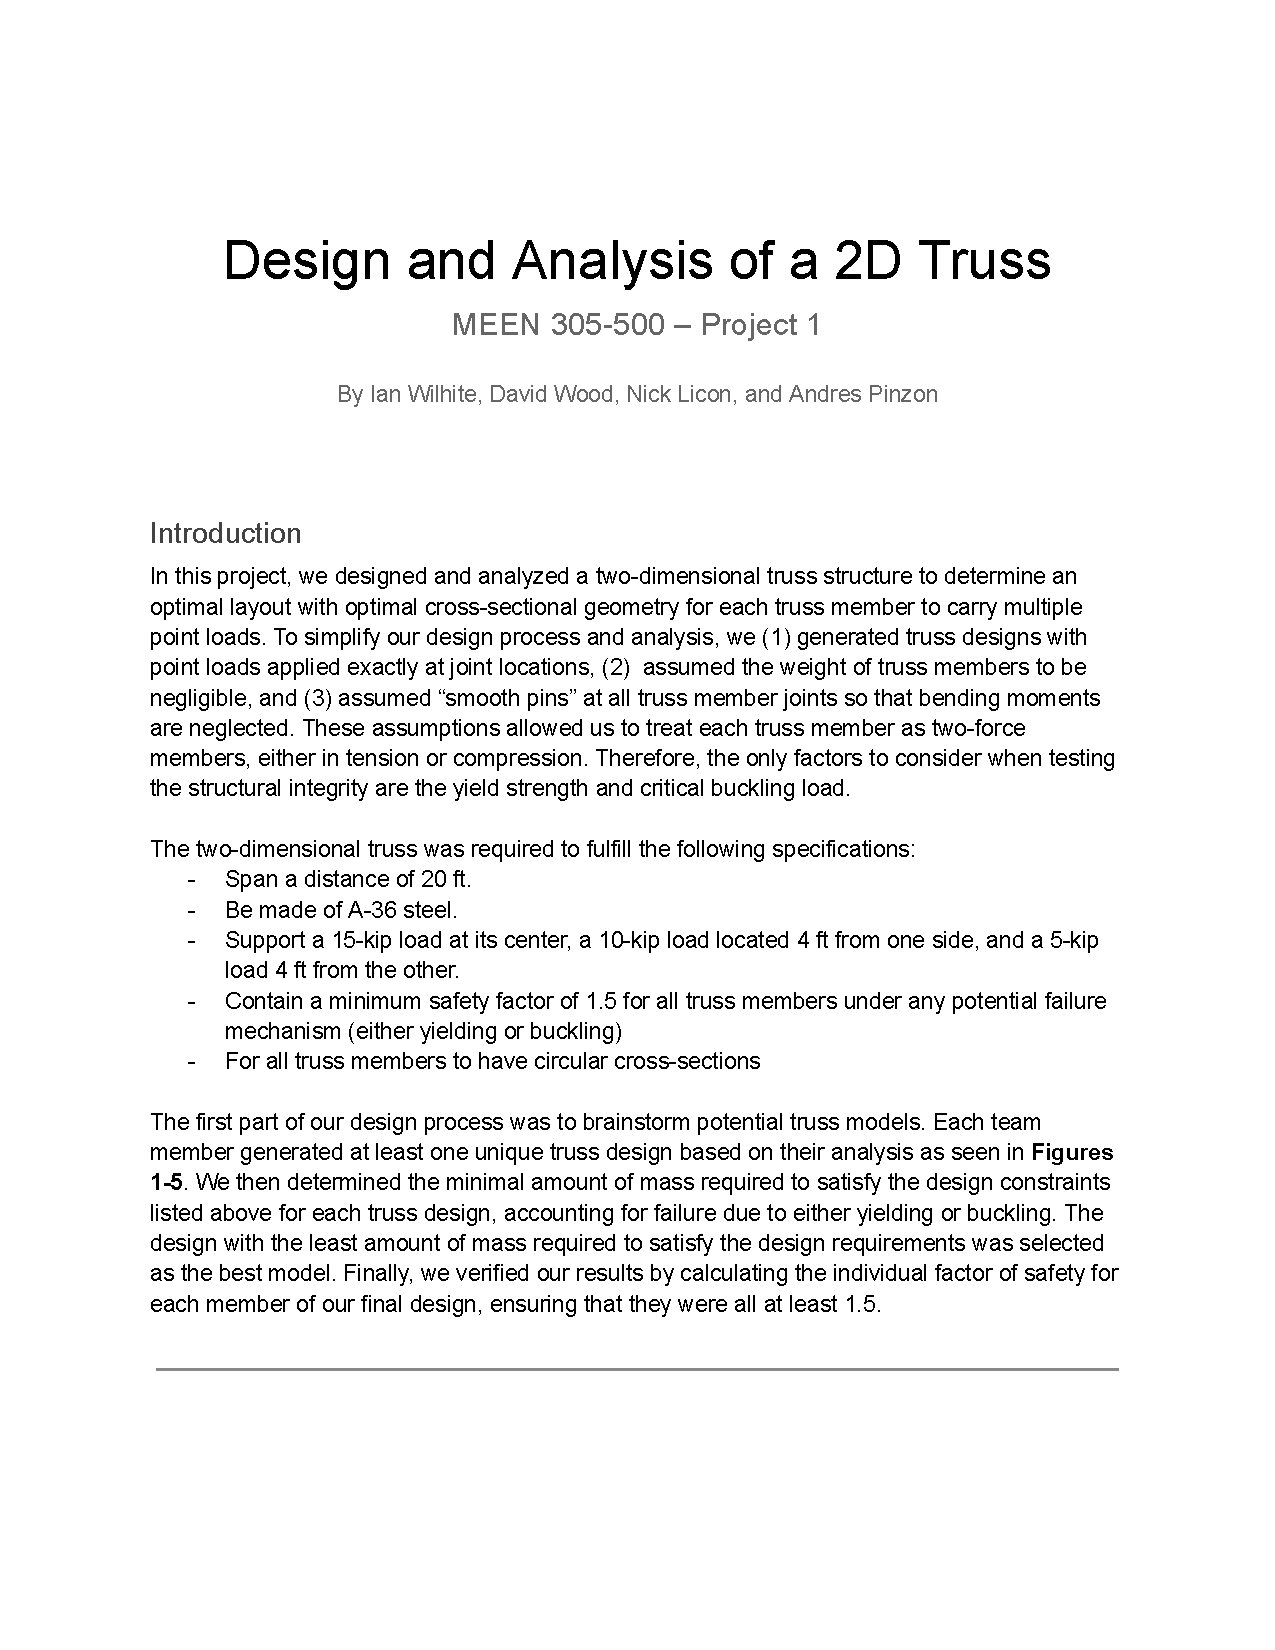
\includepdf[pages=-]{\detokenize{Resources/meen-305/meen-305-Project_1.pdf}}
\includepdf[pages=-]{\detokenize{Resources/meen-305/meen-305-Project_2.pdf}}

\hyperlink{toc}{Back to Contents}
\section{Interdisciplinary Engineering ABET Requirements}
\subsection*{Summary}
\textbf{Content:} This section includes documents fulfilling the ABET requirements for the Interdisciplinary Engineering program (ITDE 201).
\begin{itemize}
    \item itde-201-ECS.pdf (Engineering Career Skills)
    \item itde-201-PDP.pdf (Professional Development Plan)
\end{itemize}
\textbf{Contributors:} Ian Wilhite (Solo Project)

\textbf{Key Skills:} Professional Development, Career Planning, Engineering Ethics, ABET Accreditation, Lifelong Learning.

\textbf{Relevance:} These documents showcase a commitment to professional growth and an understanding of the ethical and professional responsibilities of an engineer, as outlined by ABET.

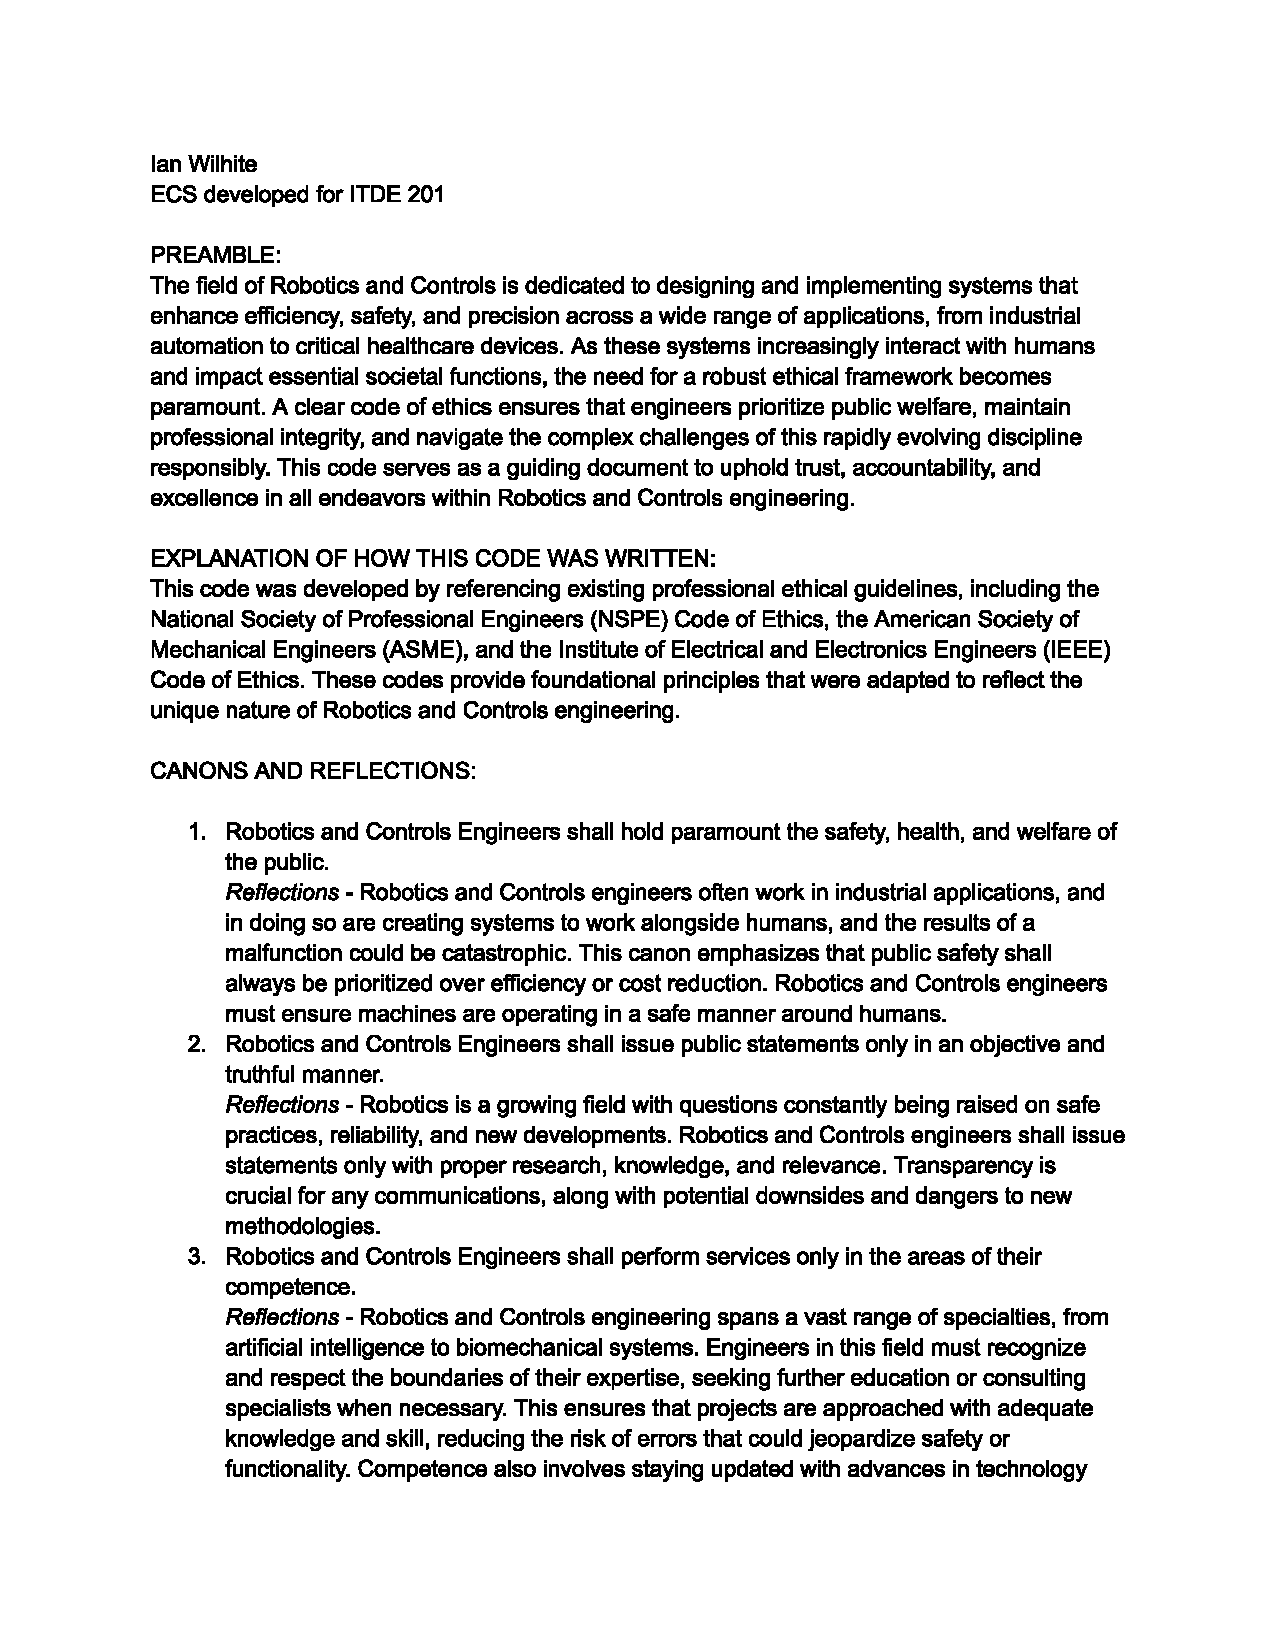
\includepdf[pages=-]{\detokenize{Resources/itde-201/itde-201-ECS.pdf}}
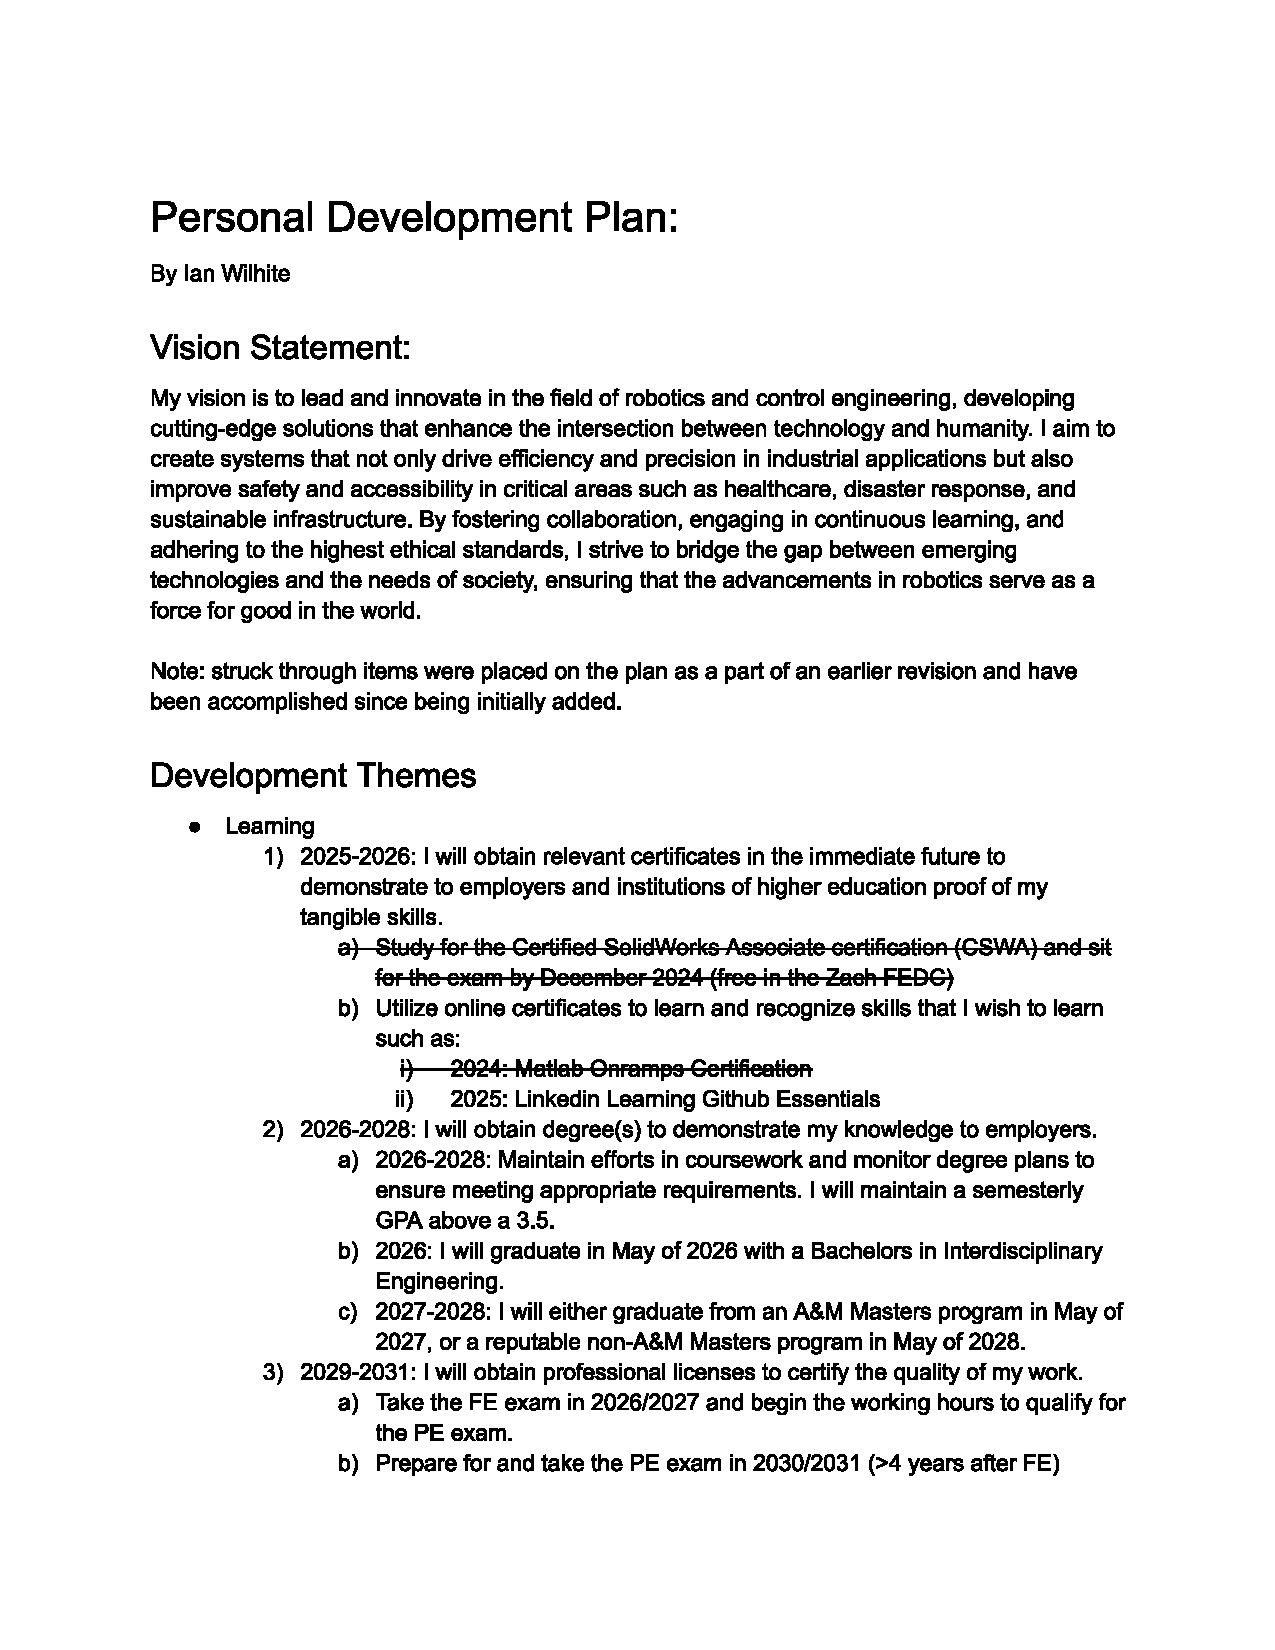
\includepdf[pages=-]{\detokenize{Resources/itde-201/itde-201-PDP.pdf}}

\hyperlink{toc}{Back to Contents}
\section{NSF Grand Challenges Scholars Program (GCSP)}
\subsection*{Summary}
\textbf{Content:} This section presents work from the NSF Grand Challenges Scholars Program (ENGR 499), including documentation of outside activities and a final presentation.
\begin{itemize}
    \item engr-499-outside\_activities-1.pdf
    \item engr-499-outside\_activities-2.pdf
    \item engr-499-Final\_Presentation.pdf
\end{itemize}
\textbf{Contributors:} Ian Wilhite (Solo Project)

\textbf{Key Skills:} Interdisciplinary Research, Global Challenges, Societal Impact, Innovation, Entrepreneurial Mindset, Research Communication.

\textbf{Relevance:} Participation in this prestigious program demonstrates a commitment to addressing major global challenges through an interdisciplinary and entrepreneurial approach.
vs

\hyperlink{toc}{Back to Contents}
\section{NASA L'SPACE Mission Concept Academy (MCA)}
\subsection*{Summary}
\textbf{Content:} This section contains the Mission Concept Review (MCR) and System Requirements Review (SRR) documents from the NASA L'SPACE Mission Concept Academy.
\begin{itemize}
    \item LSPACE-MCA\_TEAM\_01\_MCR.pdf
    \item LSPACE-MCA\_TEAM\_01\_SRR.pdf
\end{itemize}
\textbf{Contributors:} Team 01 (Team Project)

\textbf{Key Skills:} Systems Engineering, Mission Design, NASA Project Lifecycle, Requirements Engineering, Mission Concept Development, Team Collaboration.

\textbf{Relevance:} This experience provides direct insight into NASA's mission development process, demonstrating the ability to work in a team to develop a mission concept and its associated requirements in a structured, professional environment.

\includepdf[pages=-]{\detokenize{Resources/LSPACE/LSPACE-MCA_TEAM_01_MCR.pdf}}
\includepdf[pages=-]{\detokenize{Resources/LSPACE/LSPACE-MCA_TEAM_01_SRR.pdf}}
\includepdf[pages=-]{\detokenize{Resources/LSPACE/LSPACE-MCA_TEAM_01_MDR.pdf}}

\end{document}
